\chapter{Results}\label{sec:results}

% --------------------------------
% basic
%-----
\section{Basic equations, Laplace, Poisson, Diffusion etc.}
%-----
\section{Linear Mechanics}
%-----
\section{Nonlinear mechanics, tendon material}
%-----
\section{FEBio adapter, validation}

cook's beam

% --------------------------------
% application
\section{Application: Subcellular Models}
%-----
\section{Application: Only Fibers, Monodomain}

% fibers mesh
\begin{figure}[H]
  \centering%
  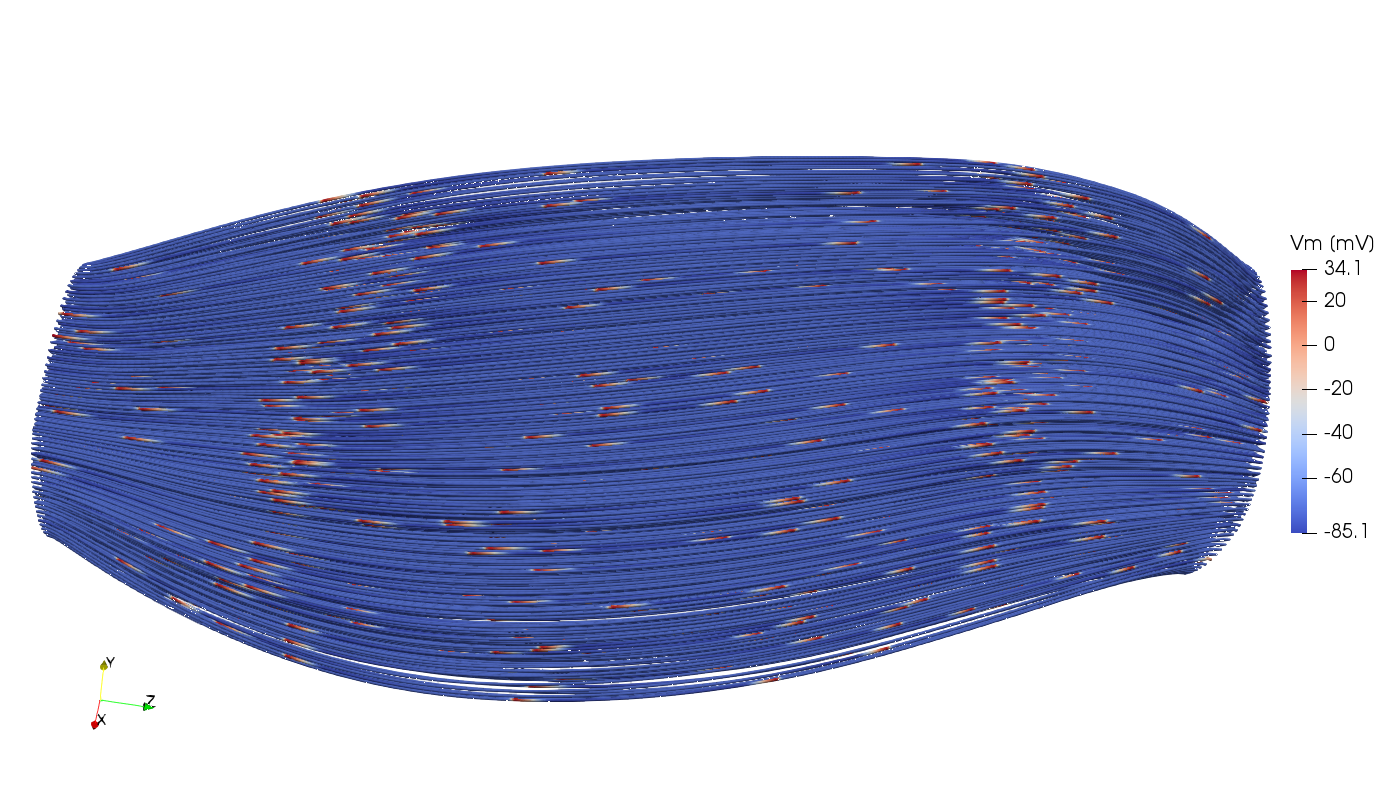
\includegraphics[width=\textwidth]{images/results/application/fibers_0.png}%
  \includegraphics[width=\textwidth]{images/results/application/fibers_1.png}%
  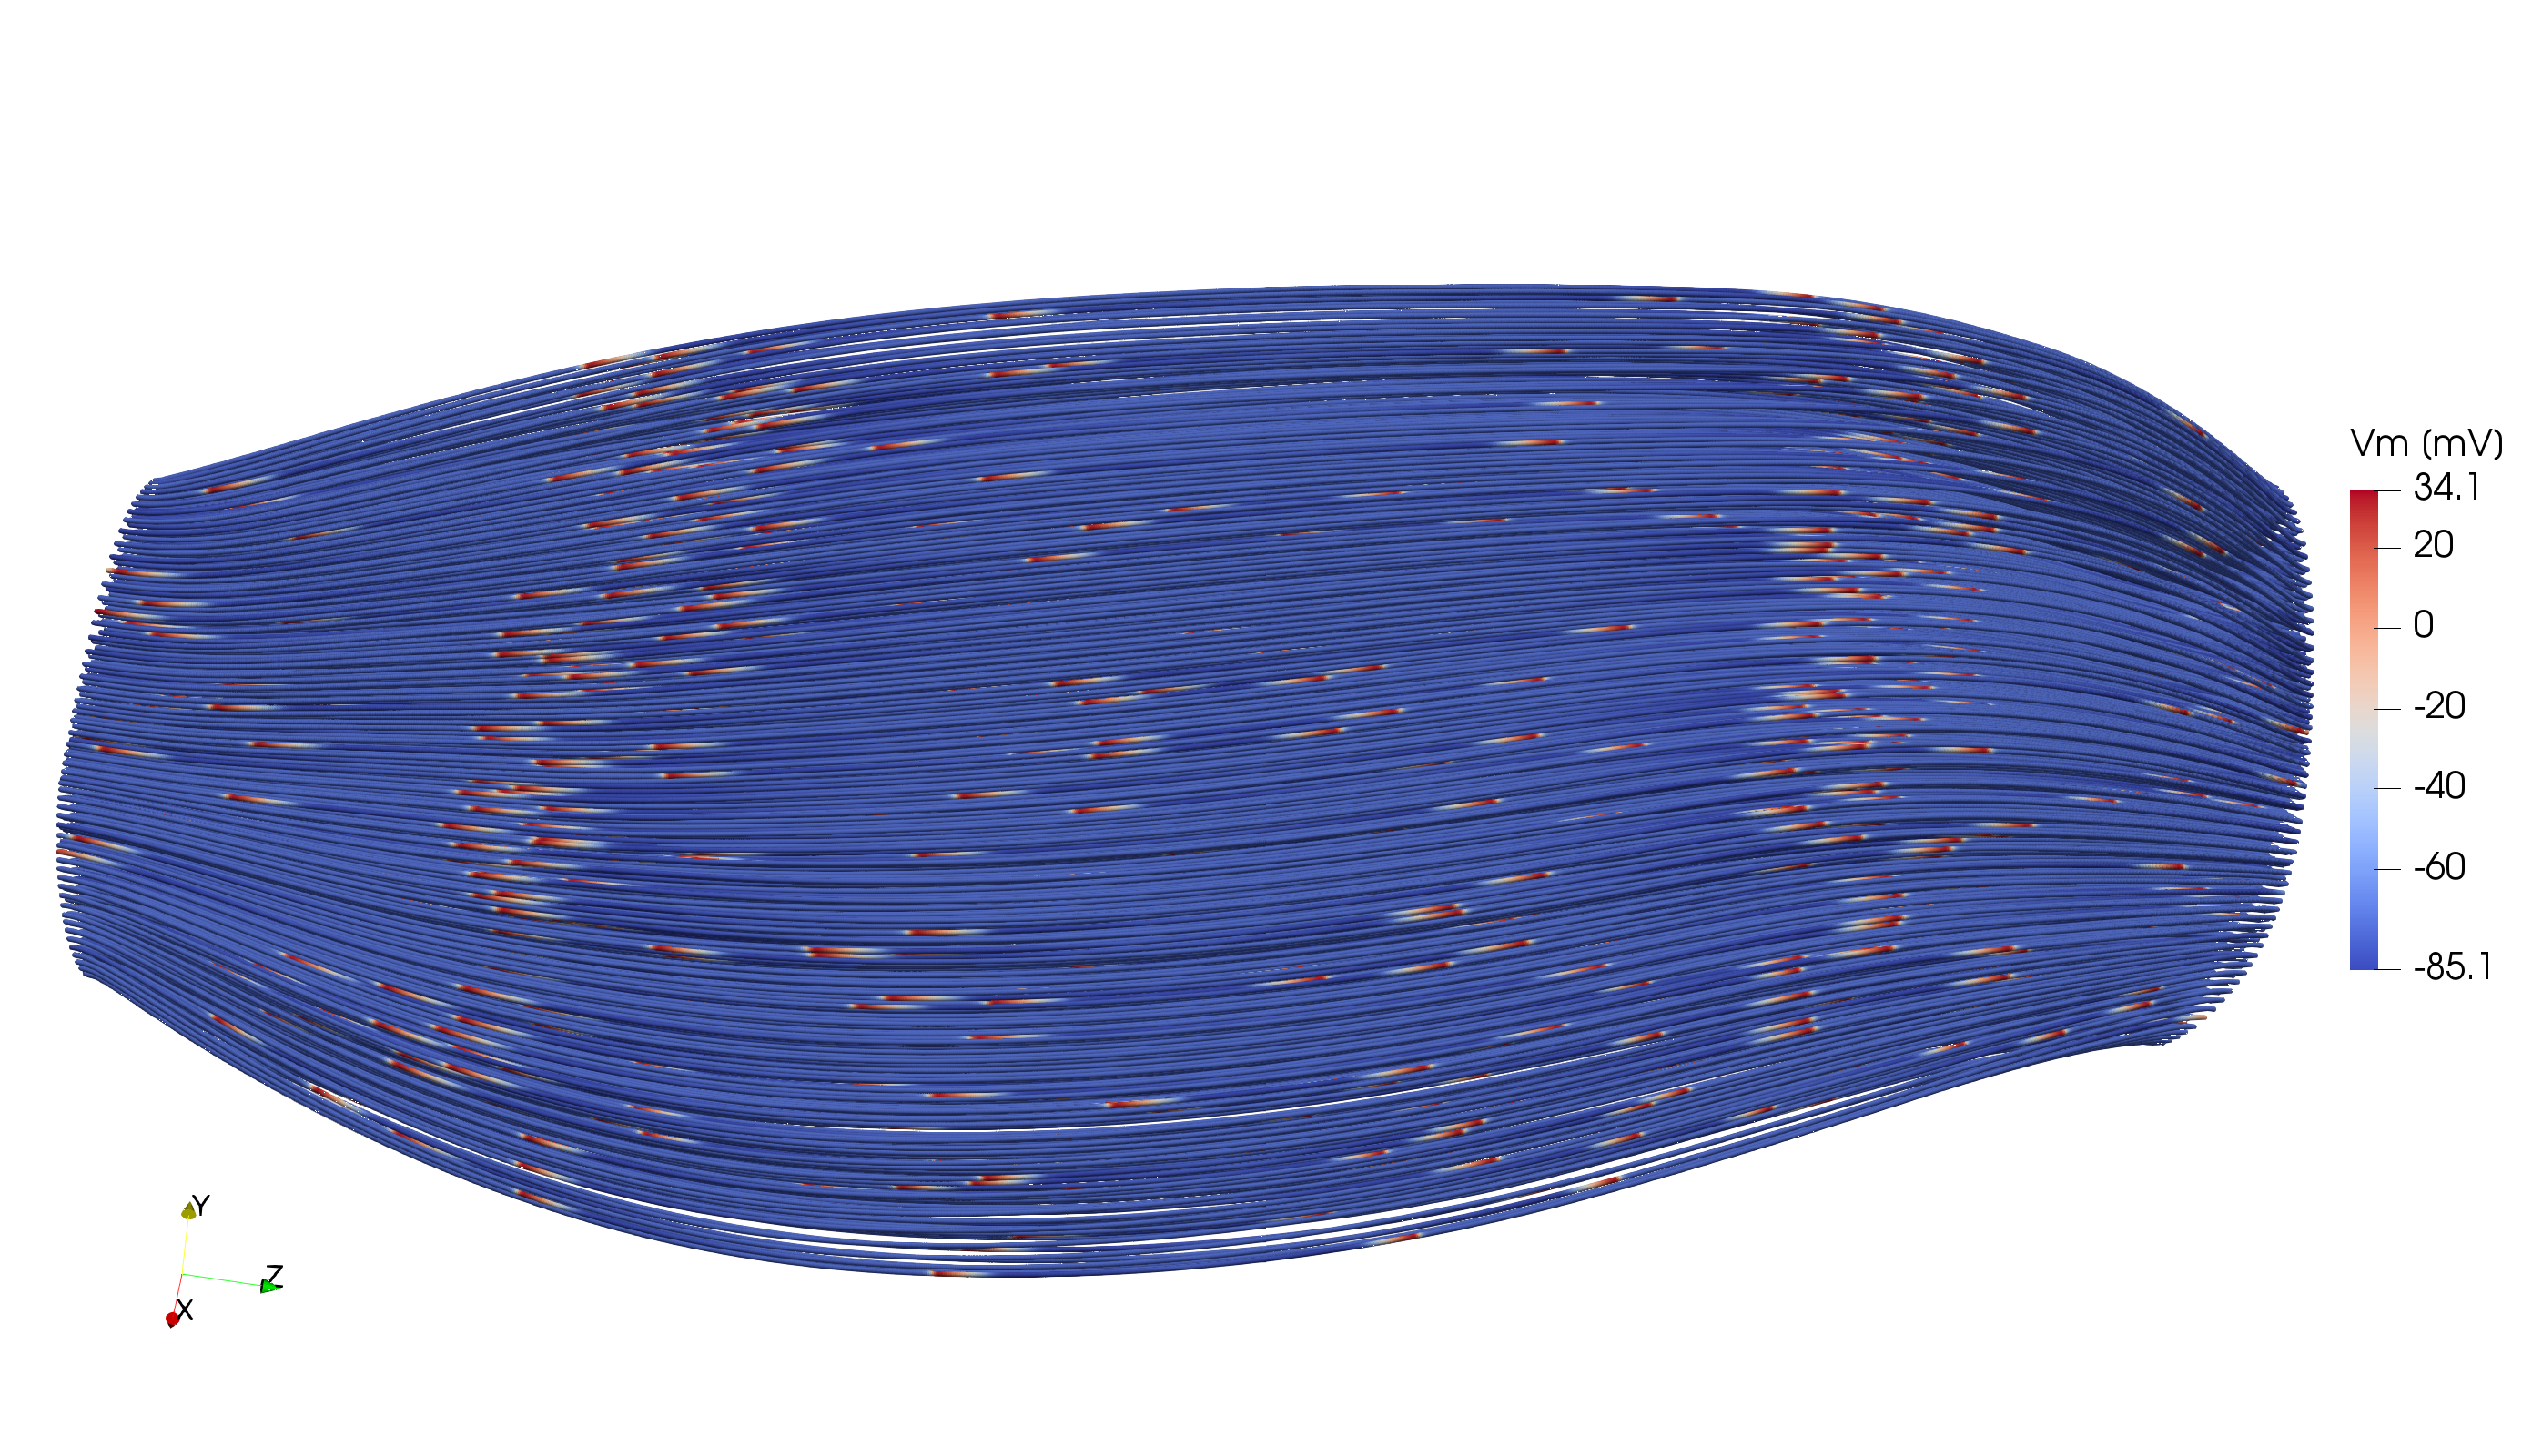
\includegraphics[width=\textwidth]{images/results/application/fibers_2.png}%
  \caption{fibers mesh}%
  \label{fig:multidomain_mesh}%
\end{figure}

%-----
\section{Application: Motoneuron with fibers}
%-----
\section{Application: Rosenfalck, artifical muscle geometry}
%-----
\section{Application: Simulation of Monodomain Fibers with EMG}

% fibers mesh
\begin{figure}[H]
  \centering%
  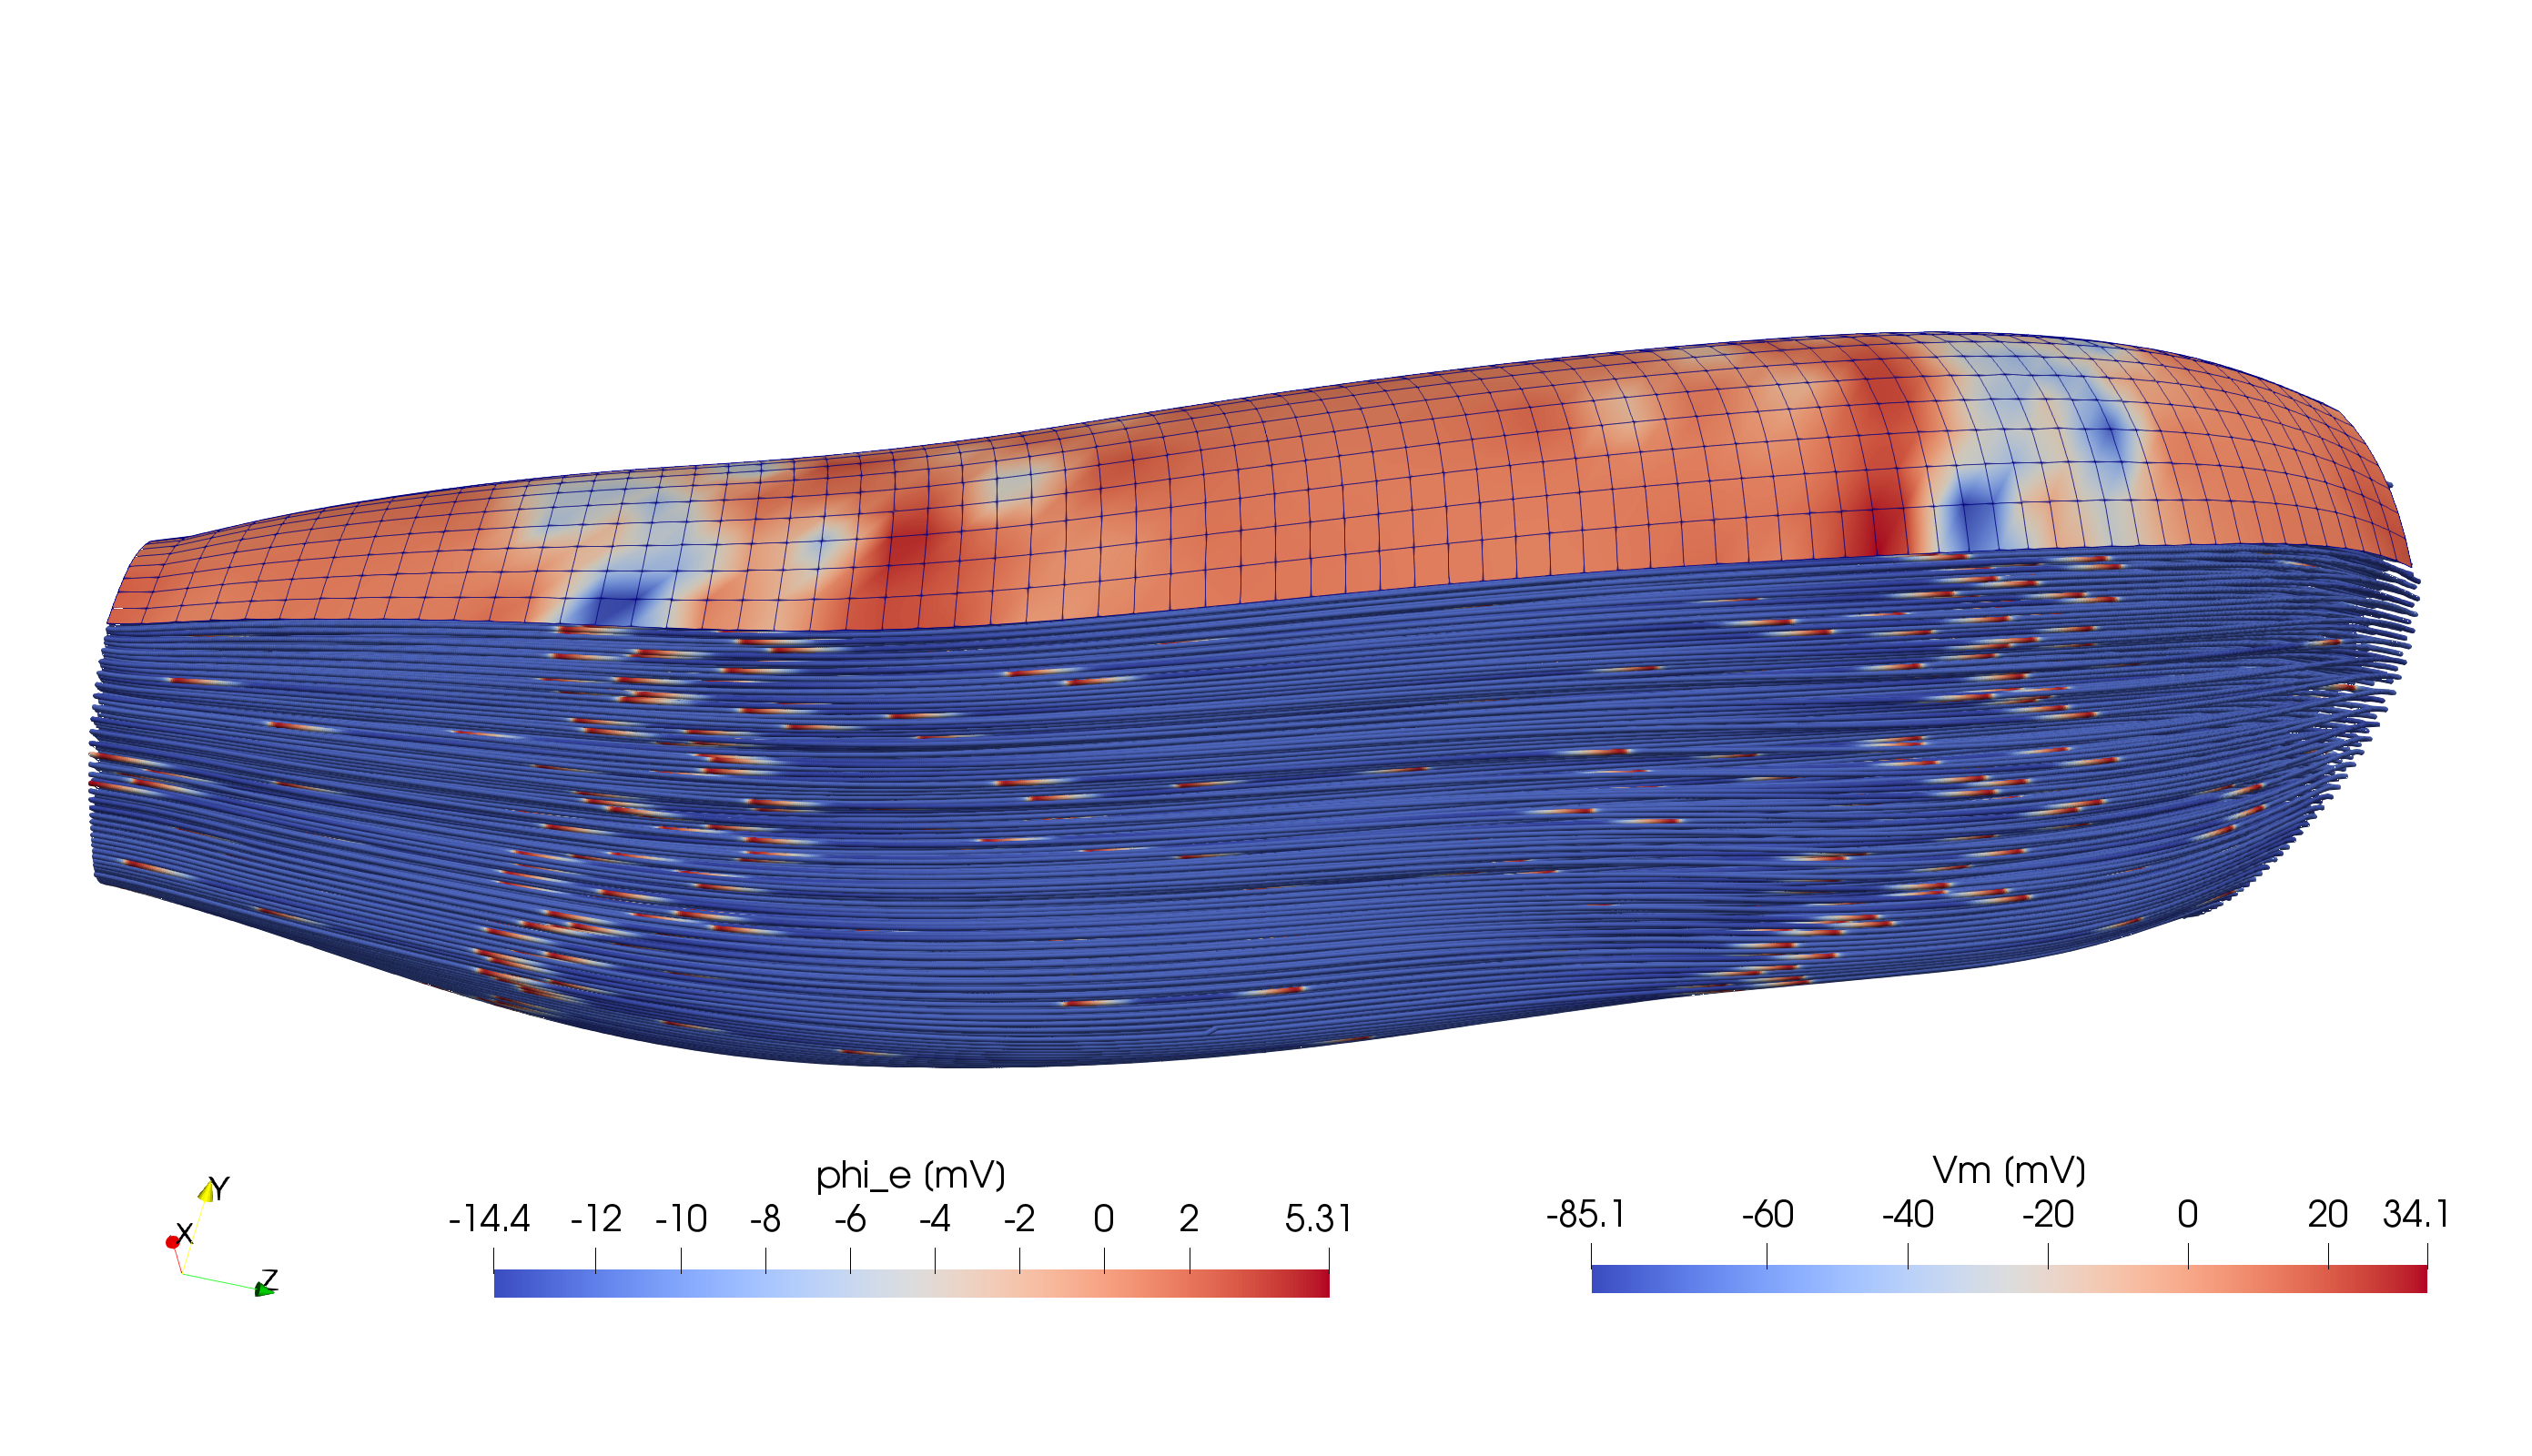
\includegraphics[width=\textwidth]{images/results/application/fibers_3.png}%
  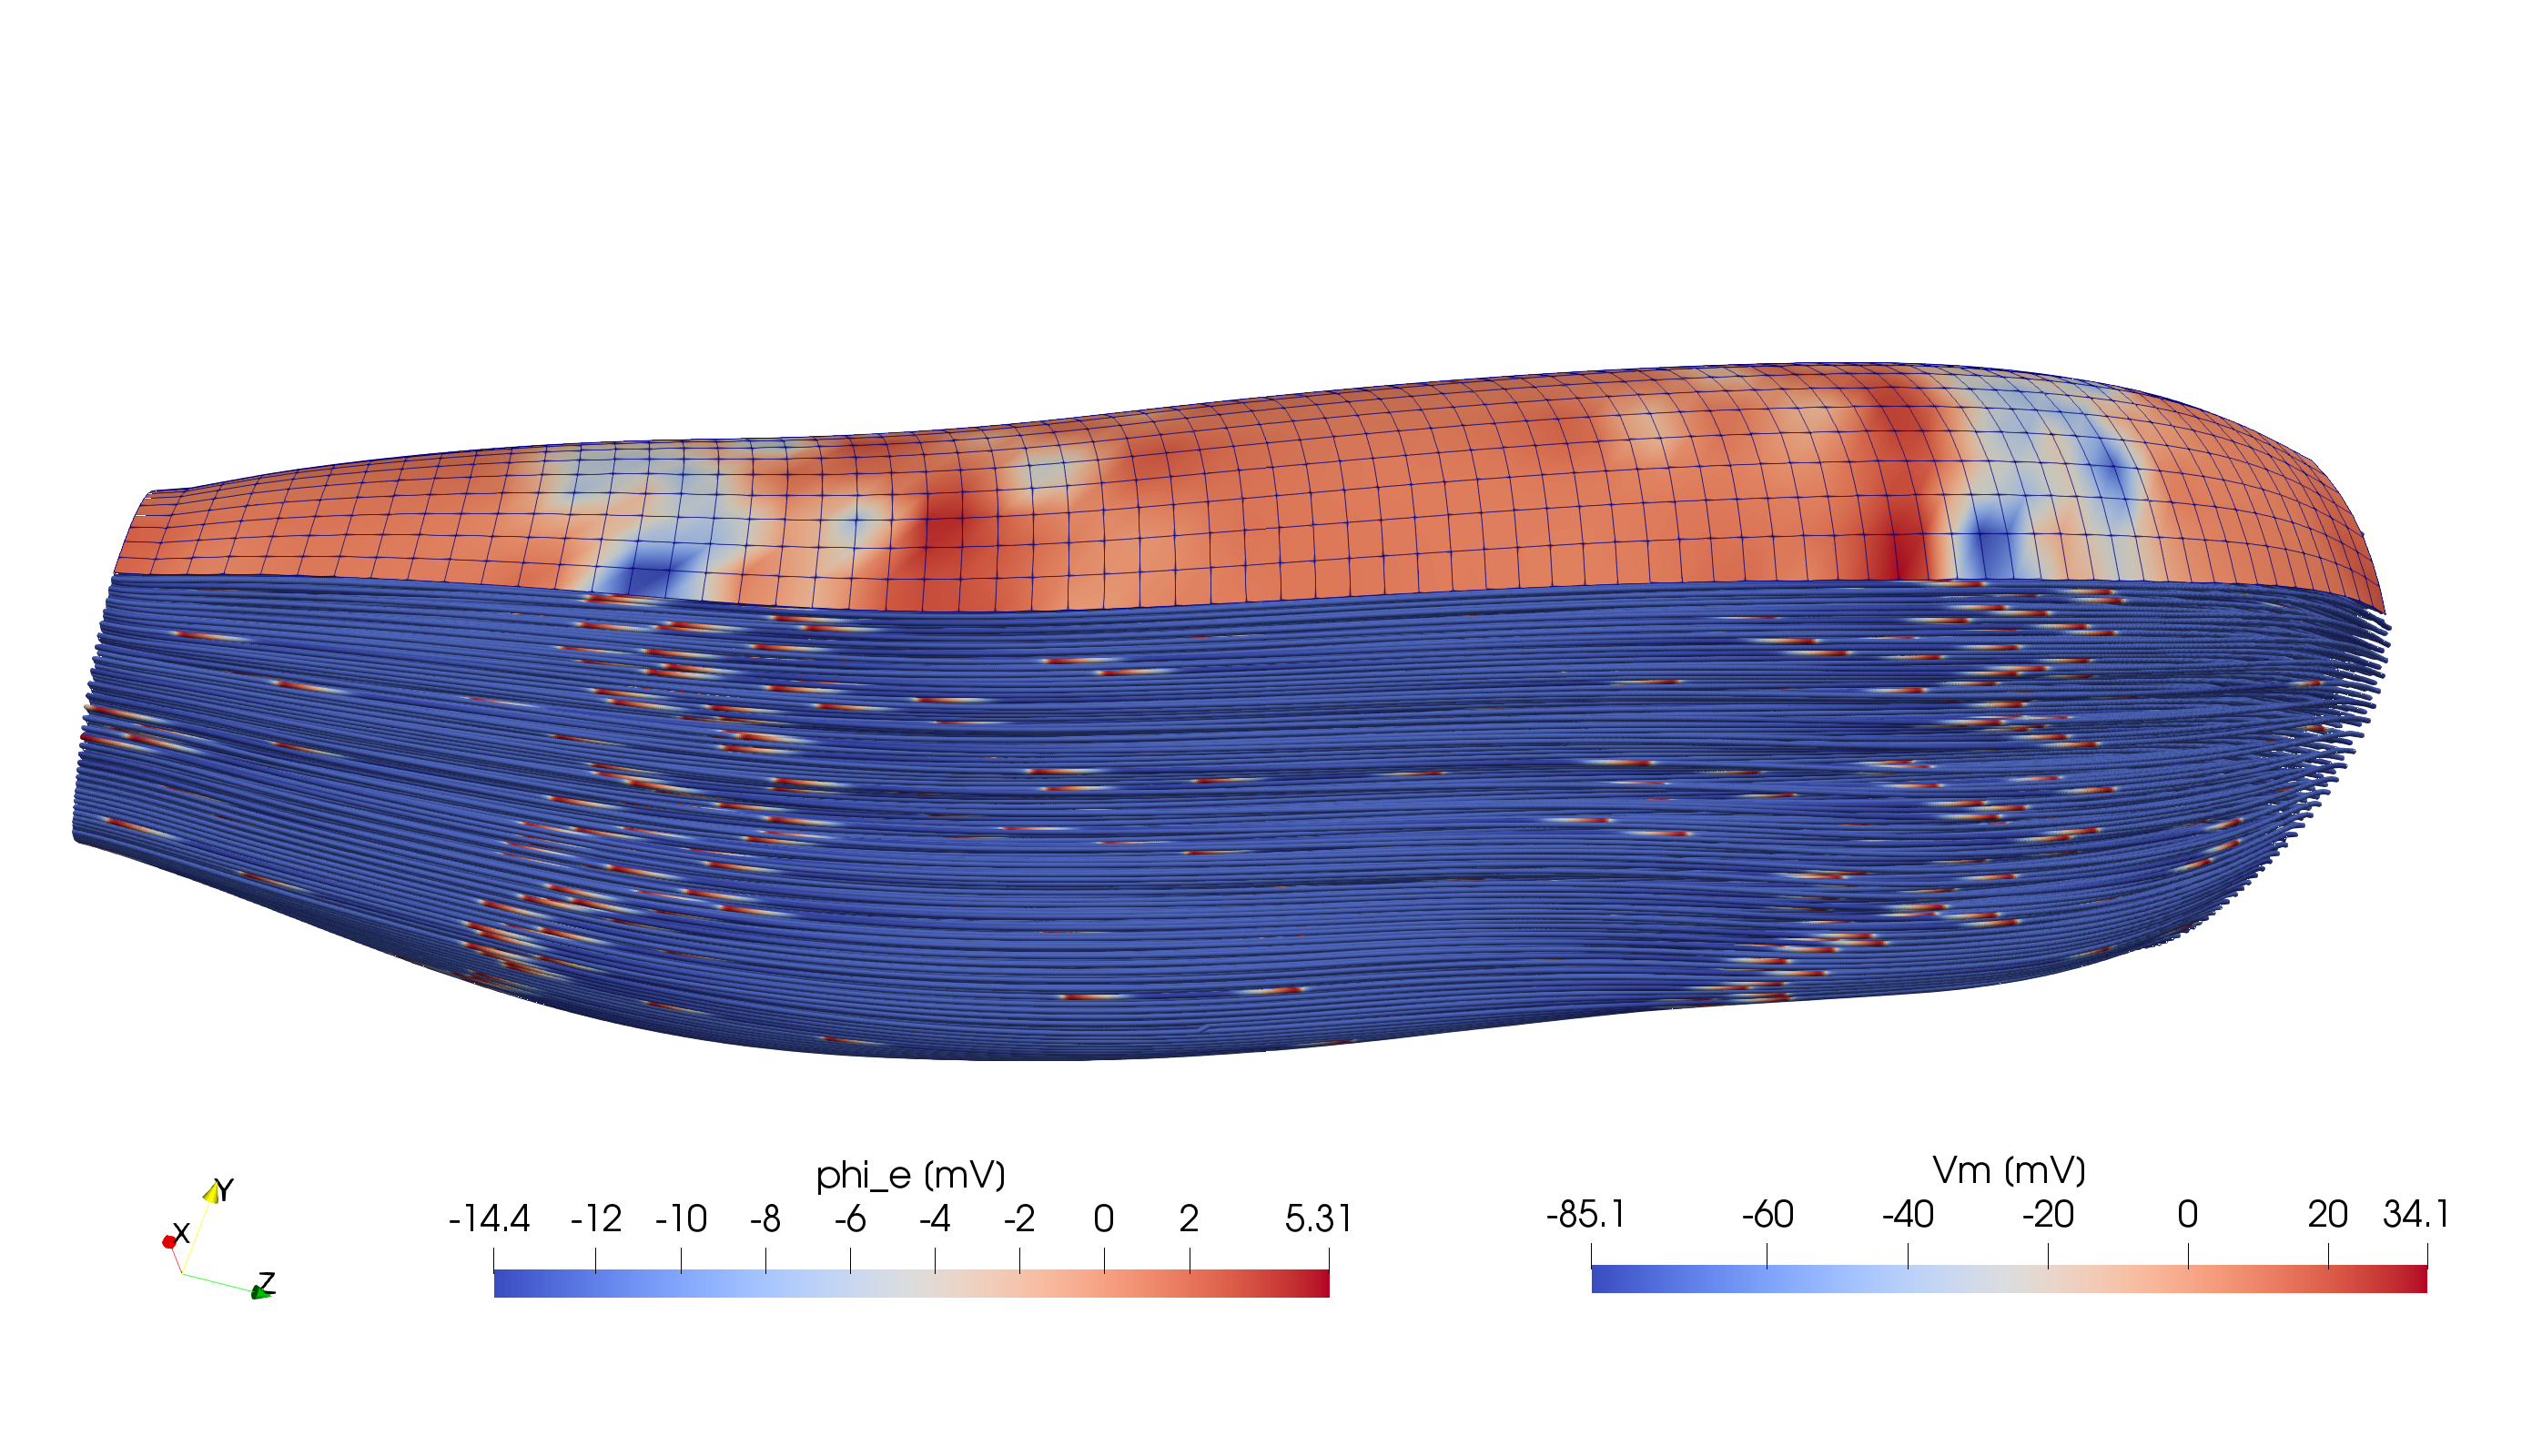
\includegraphics[width=\textwidth]{images/results/application/fibers_4.png}%
  \includegraphics[width=\textwidth]{images/results/application/fibers_5.png}%
  \caption{fibers mesh}%
  \label{fig:multidomain_mesh}%
\end{figure}


% plot of emg from fibers
\begin{figure}[H]
  \centering%
  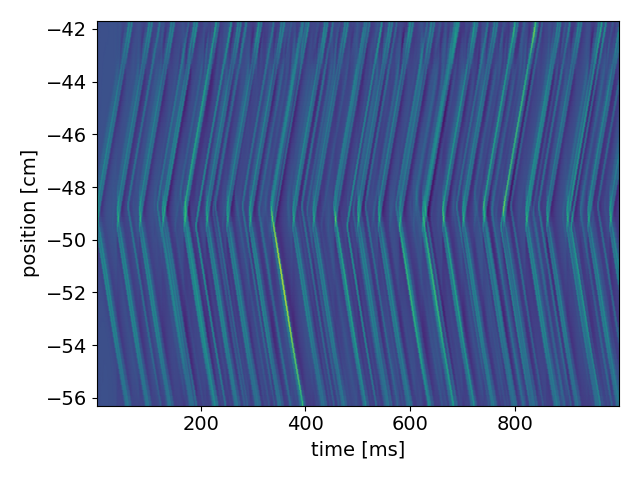
\includegraphics[width=\textwidth]{images/results/application/fibers_plot.png}%
  \caption{fibers}%
  \label{fig:fibers_plot}%
\end{figure}

% full_muscle_emg_raytrace_1.png
\begin{figure}[H]
  \centering%
  \includegraphics[width=\textwidth]{images/results/application/full_muscle_emg_raytrace_1.png}%
  \caption{muscle emg}%
  \label{fig:full_muscle_emg_raytrace_1}%
\end{figure}


%-----
\section{Application: Static bidomain}
%-----
\section{Application: Multidomain}


% multidomain fr factors
\begin{figure}[H]
  \centering%
  \begin{subfigure}[t]{0.23\textwidth}%
    \centering%
    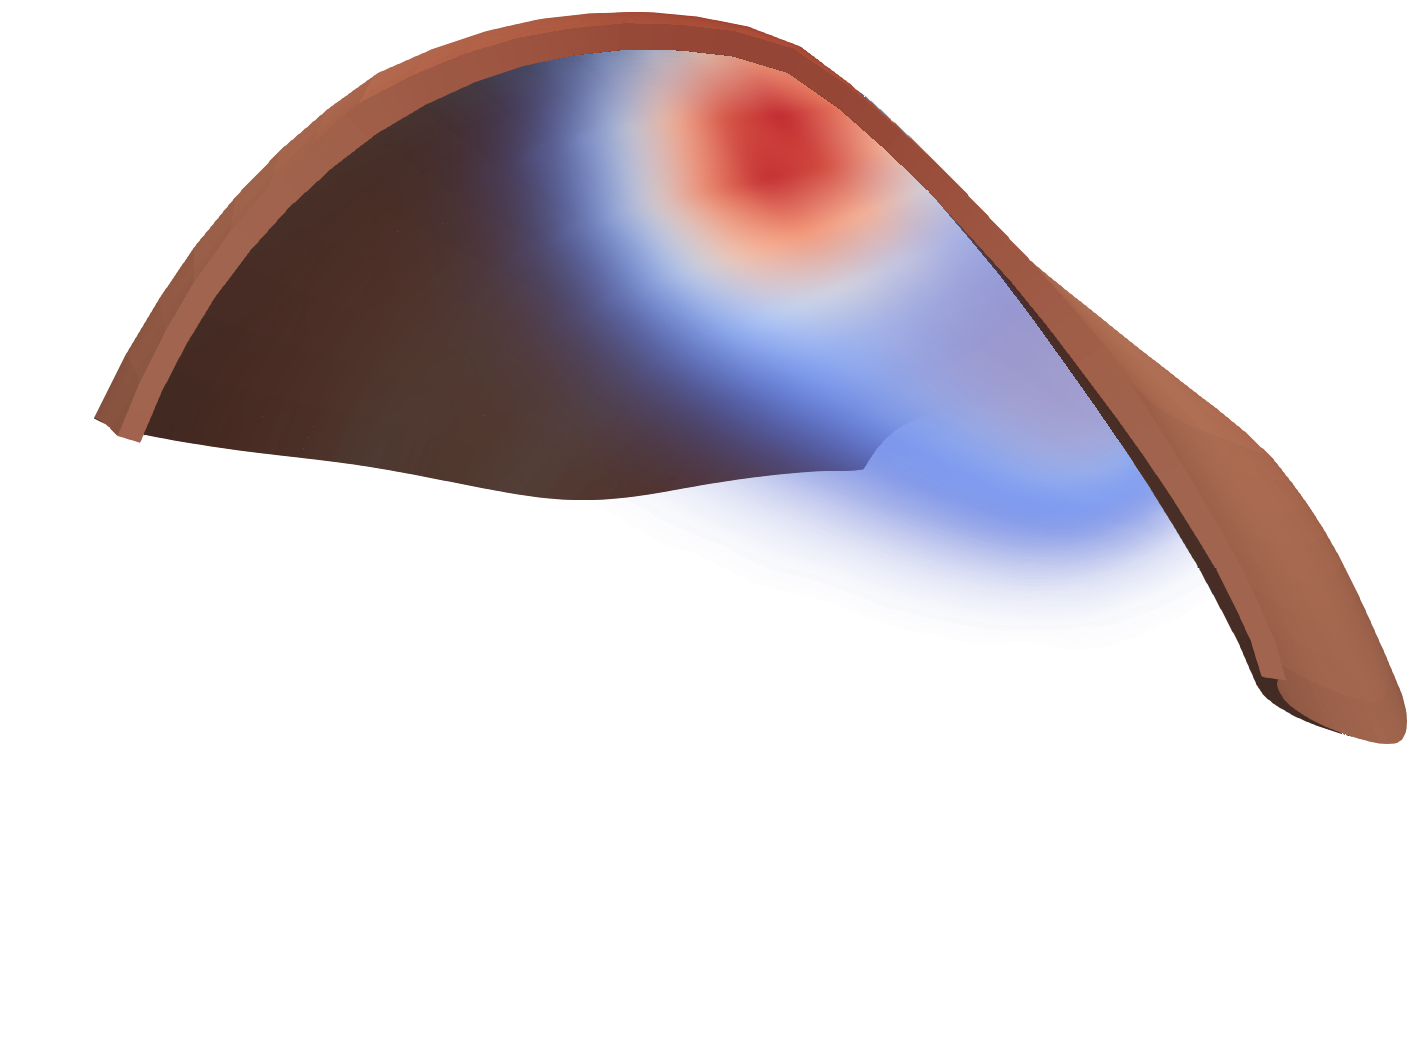
\includegraphics[width=\textwidth]{images/results/application/multidomain_fr0_cropped.png}%
    \caption{$f_r^0$}%
    \label{fig:fr0}%
  \end{subfigure}
  \,
  \begin{subfigure}[t]{0.23\textwidth}%
    \centering%
    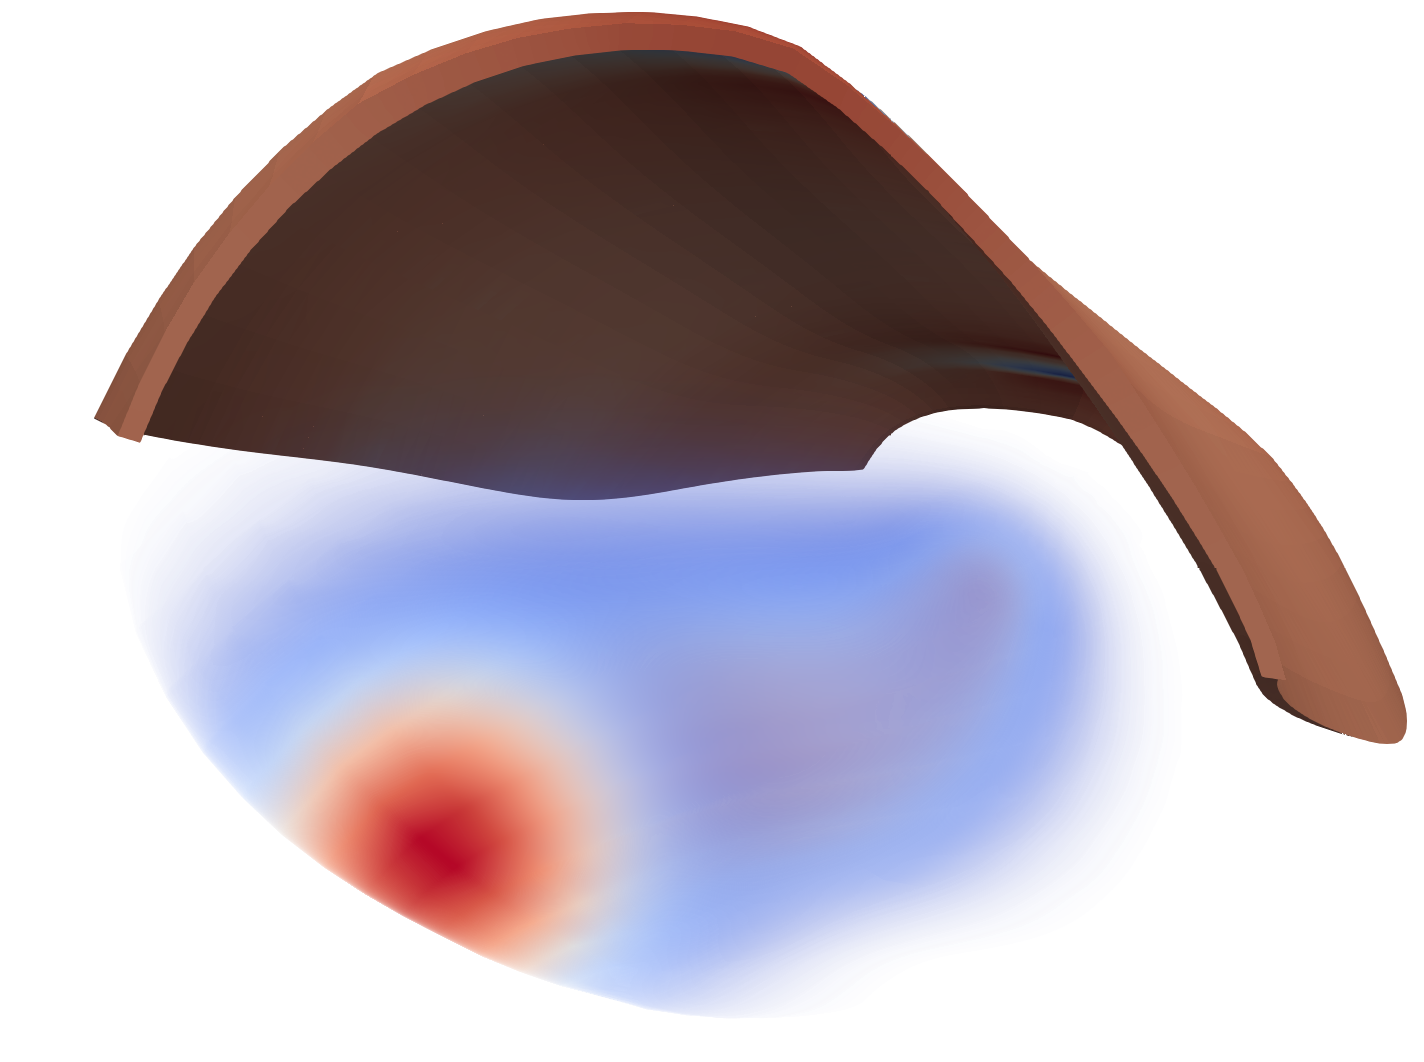
\includegraphics[width=\textwidth]{images/results/application/multidomain_fr1_cropped.png}%
    \caption{$f_r^1$}%
    \label{fig:fr1}%
  \end{subfigure}
  \,
  \begin{subfigure}[t]{0.23\textwidth}%
    \centering%
    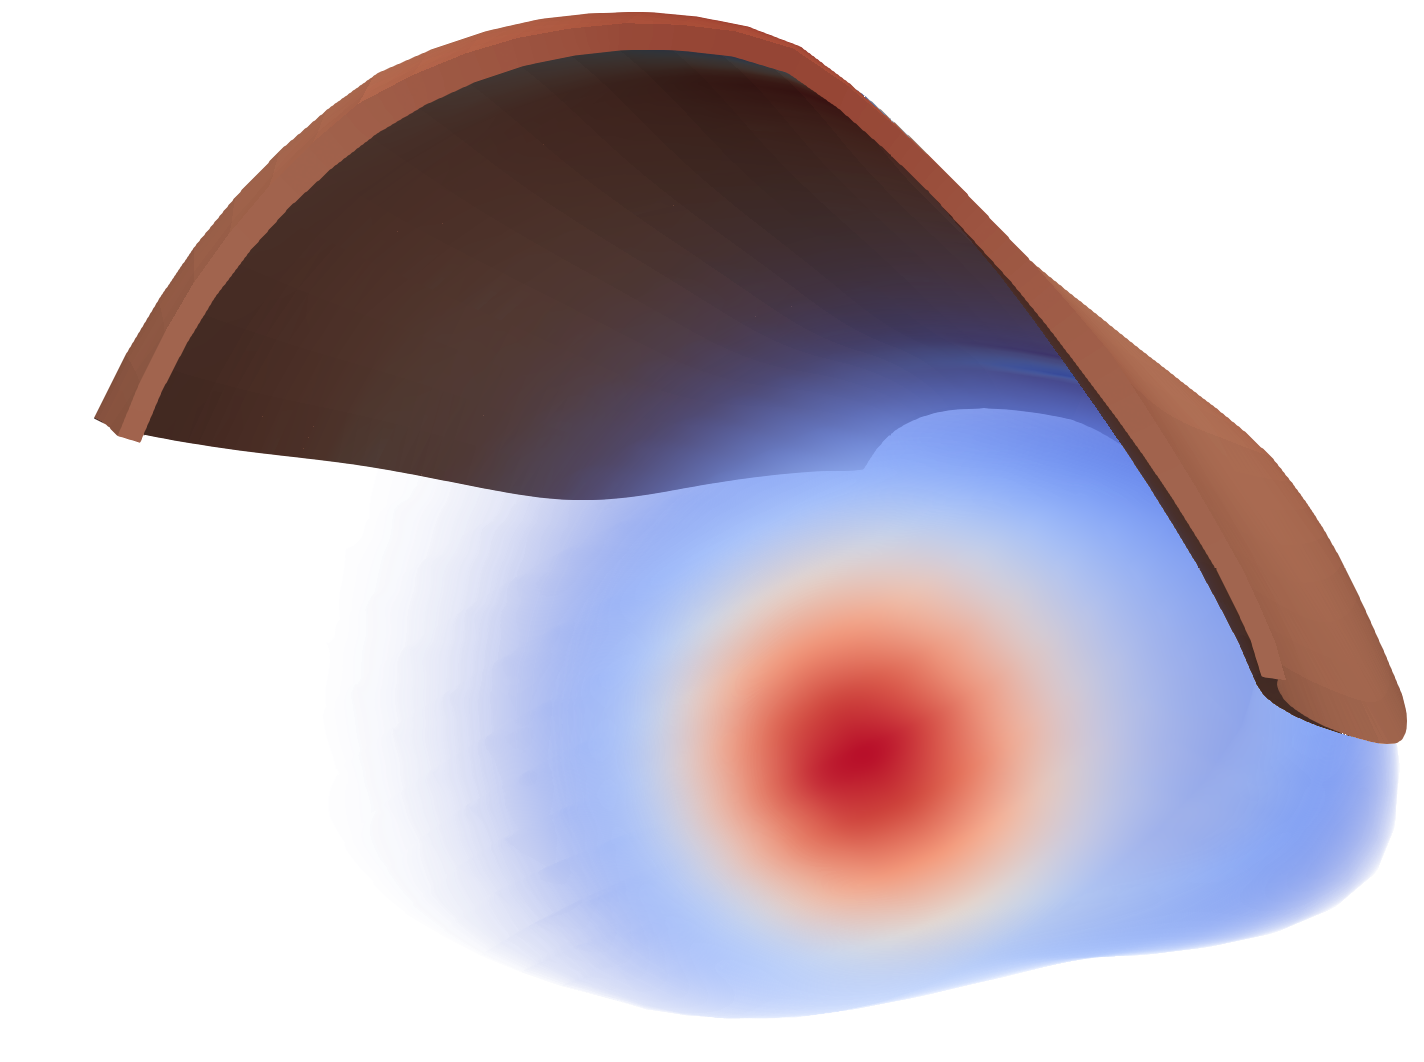
\includegraphics[width=\textwidth]{images/results/application/multidomain_fr2_cropped.png}%
    \caption{$f_r^2$}%
    \label{fig:fr2}%
  \end{subfigure}
  \,
  \begin{subfigure}[t]{0.23\textwidth}%
    \centering%
    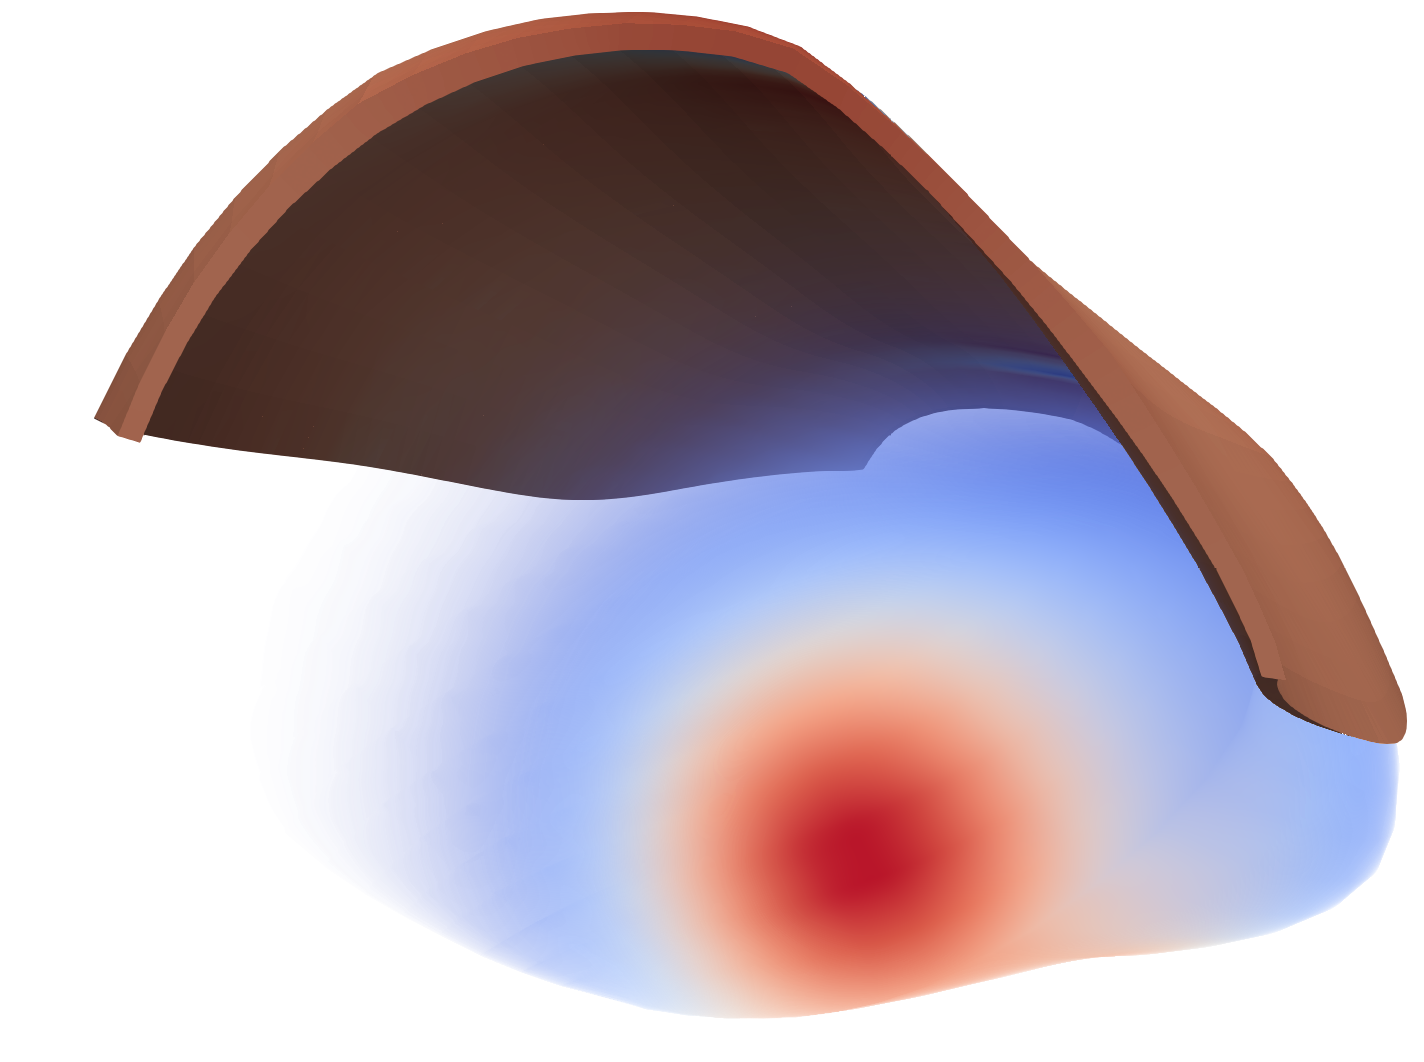
\includegraphics[width=\textwidth]{images/results/application/multidomain_fr3_cropped.png}%
    \caption{$f_r^3$}%
    \label{fig:fr3}%
  \end{subfigure}
\end{figure}%


% multidomain mesh
\begin{figure}[H]
  \centering%
  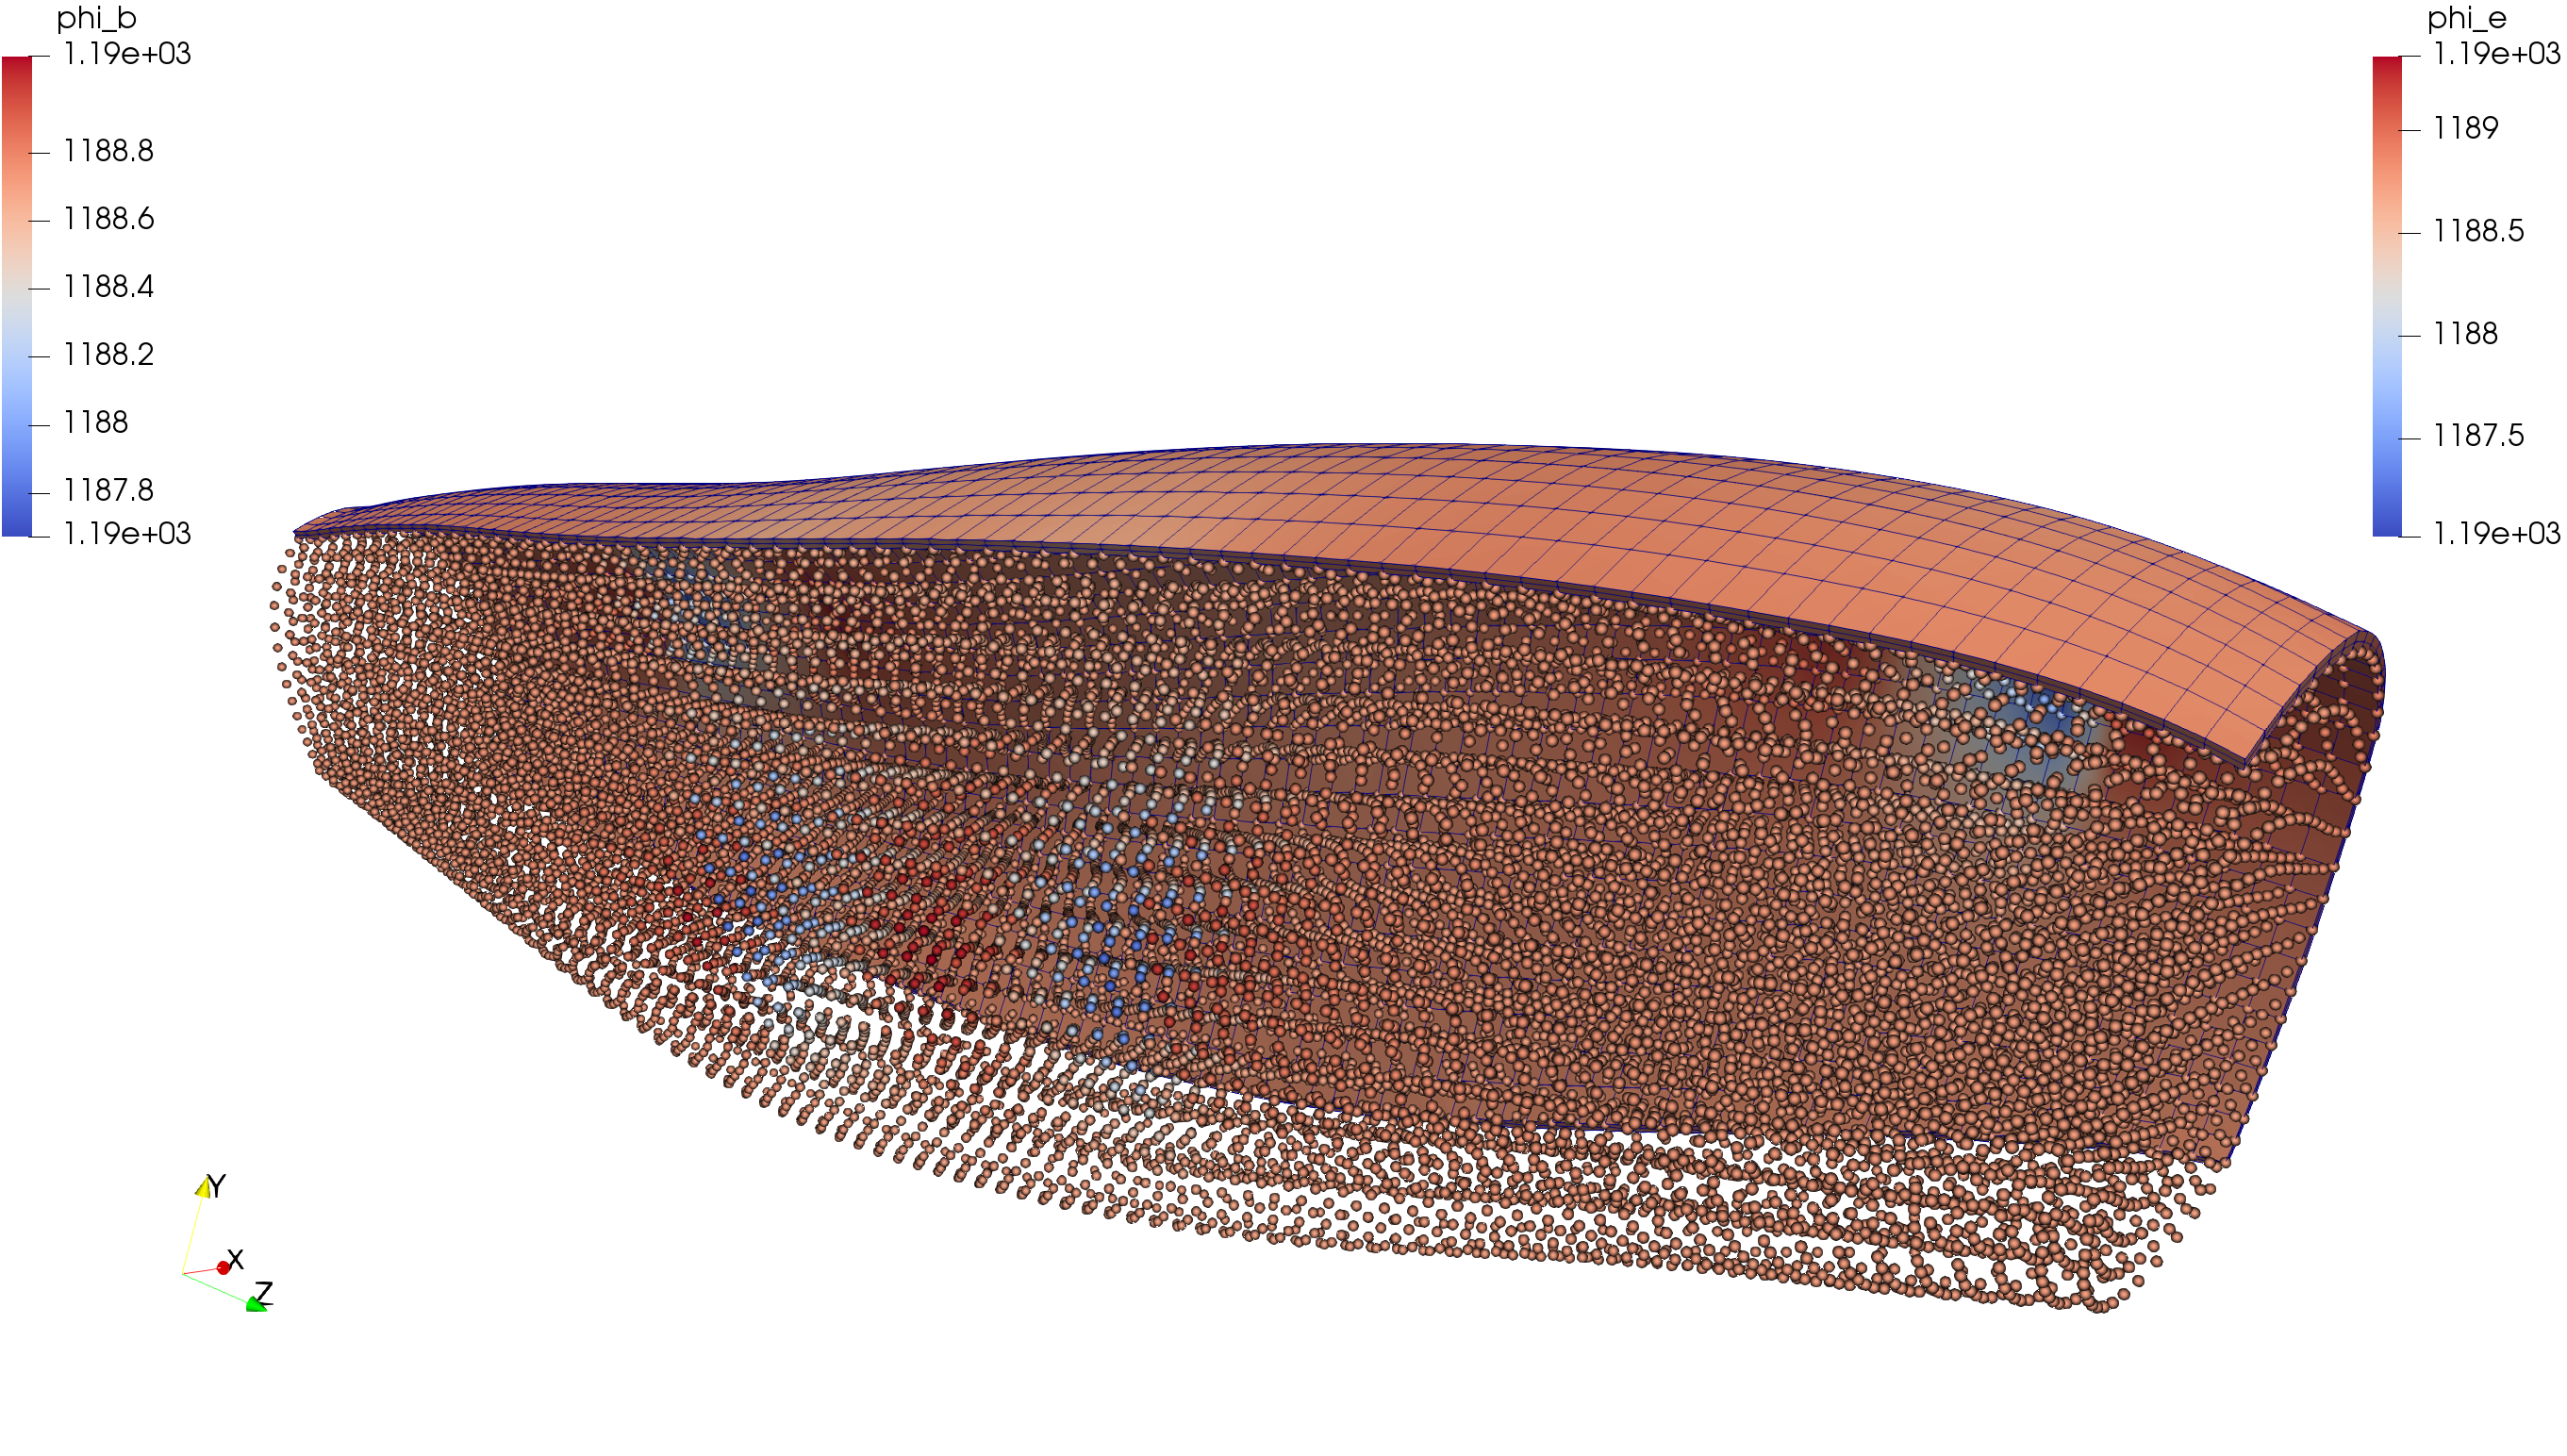
\includegraphics[width=\textwidth]{images/results/application/multidomain_mesh.png}%
  \caption{multidomain mesh}%
  \label{fig:multidomain_mesh}%
\end{figure}



% multidomain Vm
\begin{figure}[H]
  \centering%
  \begin{subfigure}[t]{\textwidth}%
    \centering%
    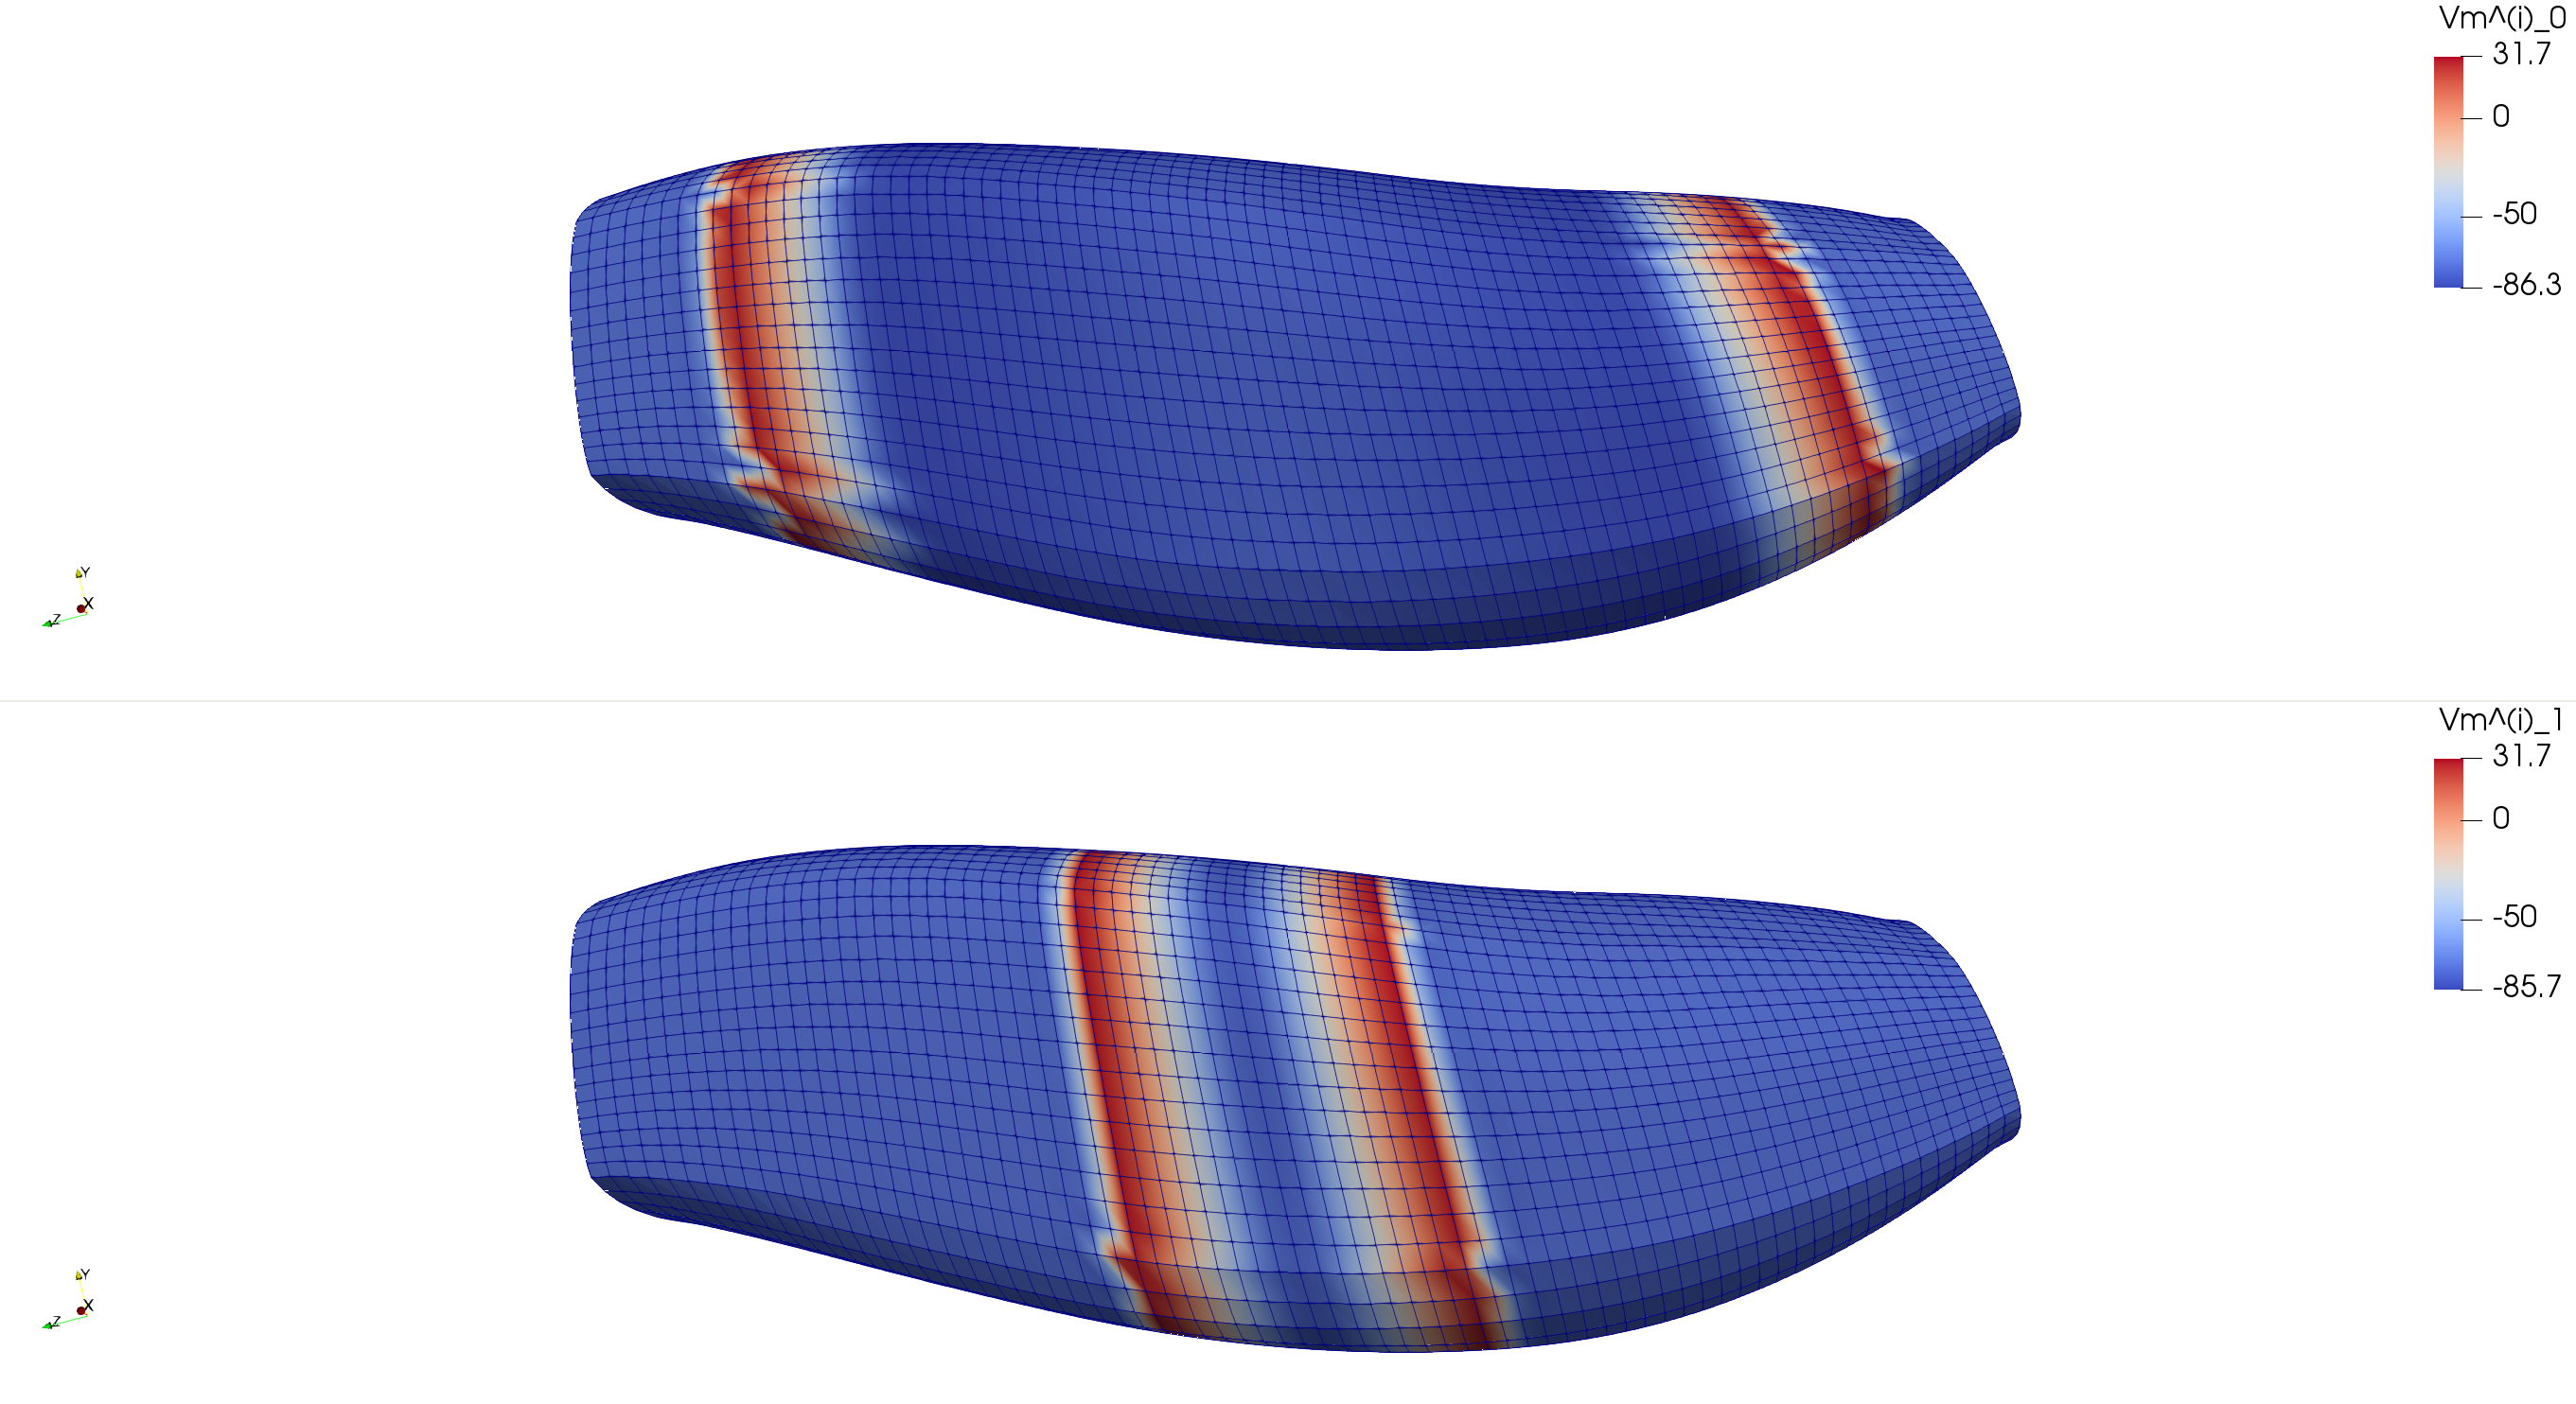
\includegraphics[width=\textwidth]{images/results/application/multidomain_Vm0_1.png}%
    \caption{$V_m^0$ and $V_m^1$}%
    \label{fig:16_hodgkin_huxley_gpu}%
  \end{subfigure} \\
  \begin{subfigure}[t]{\textwidth}%
    \centering%
    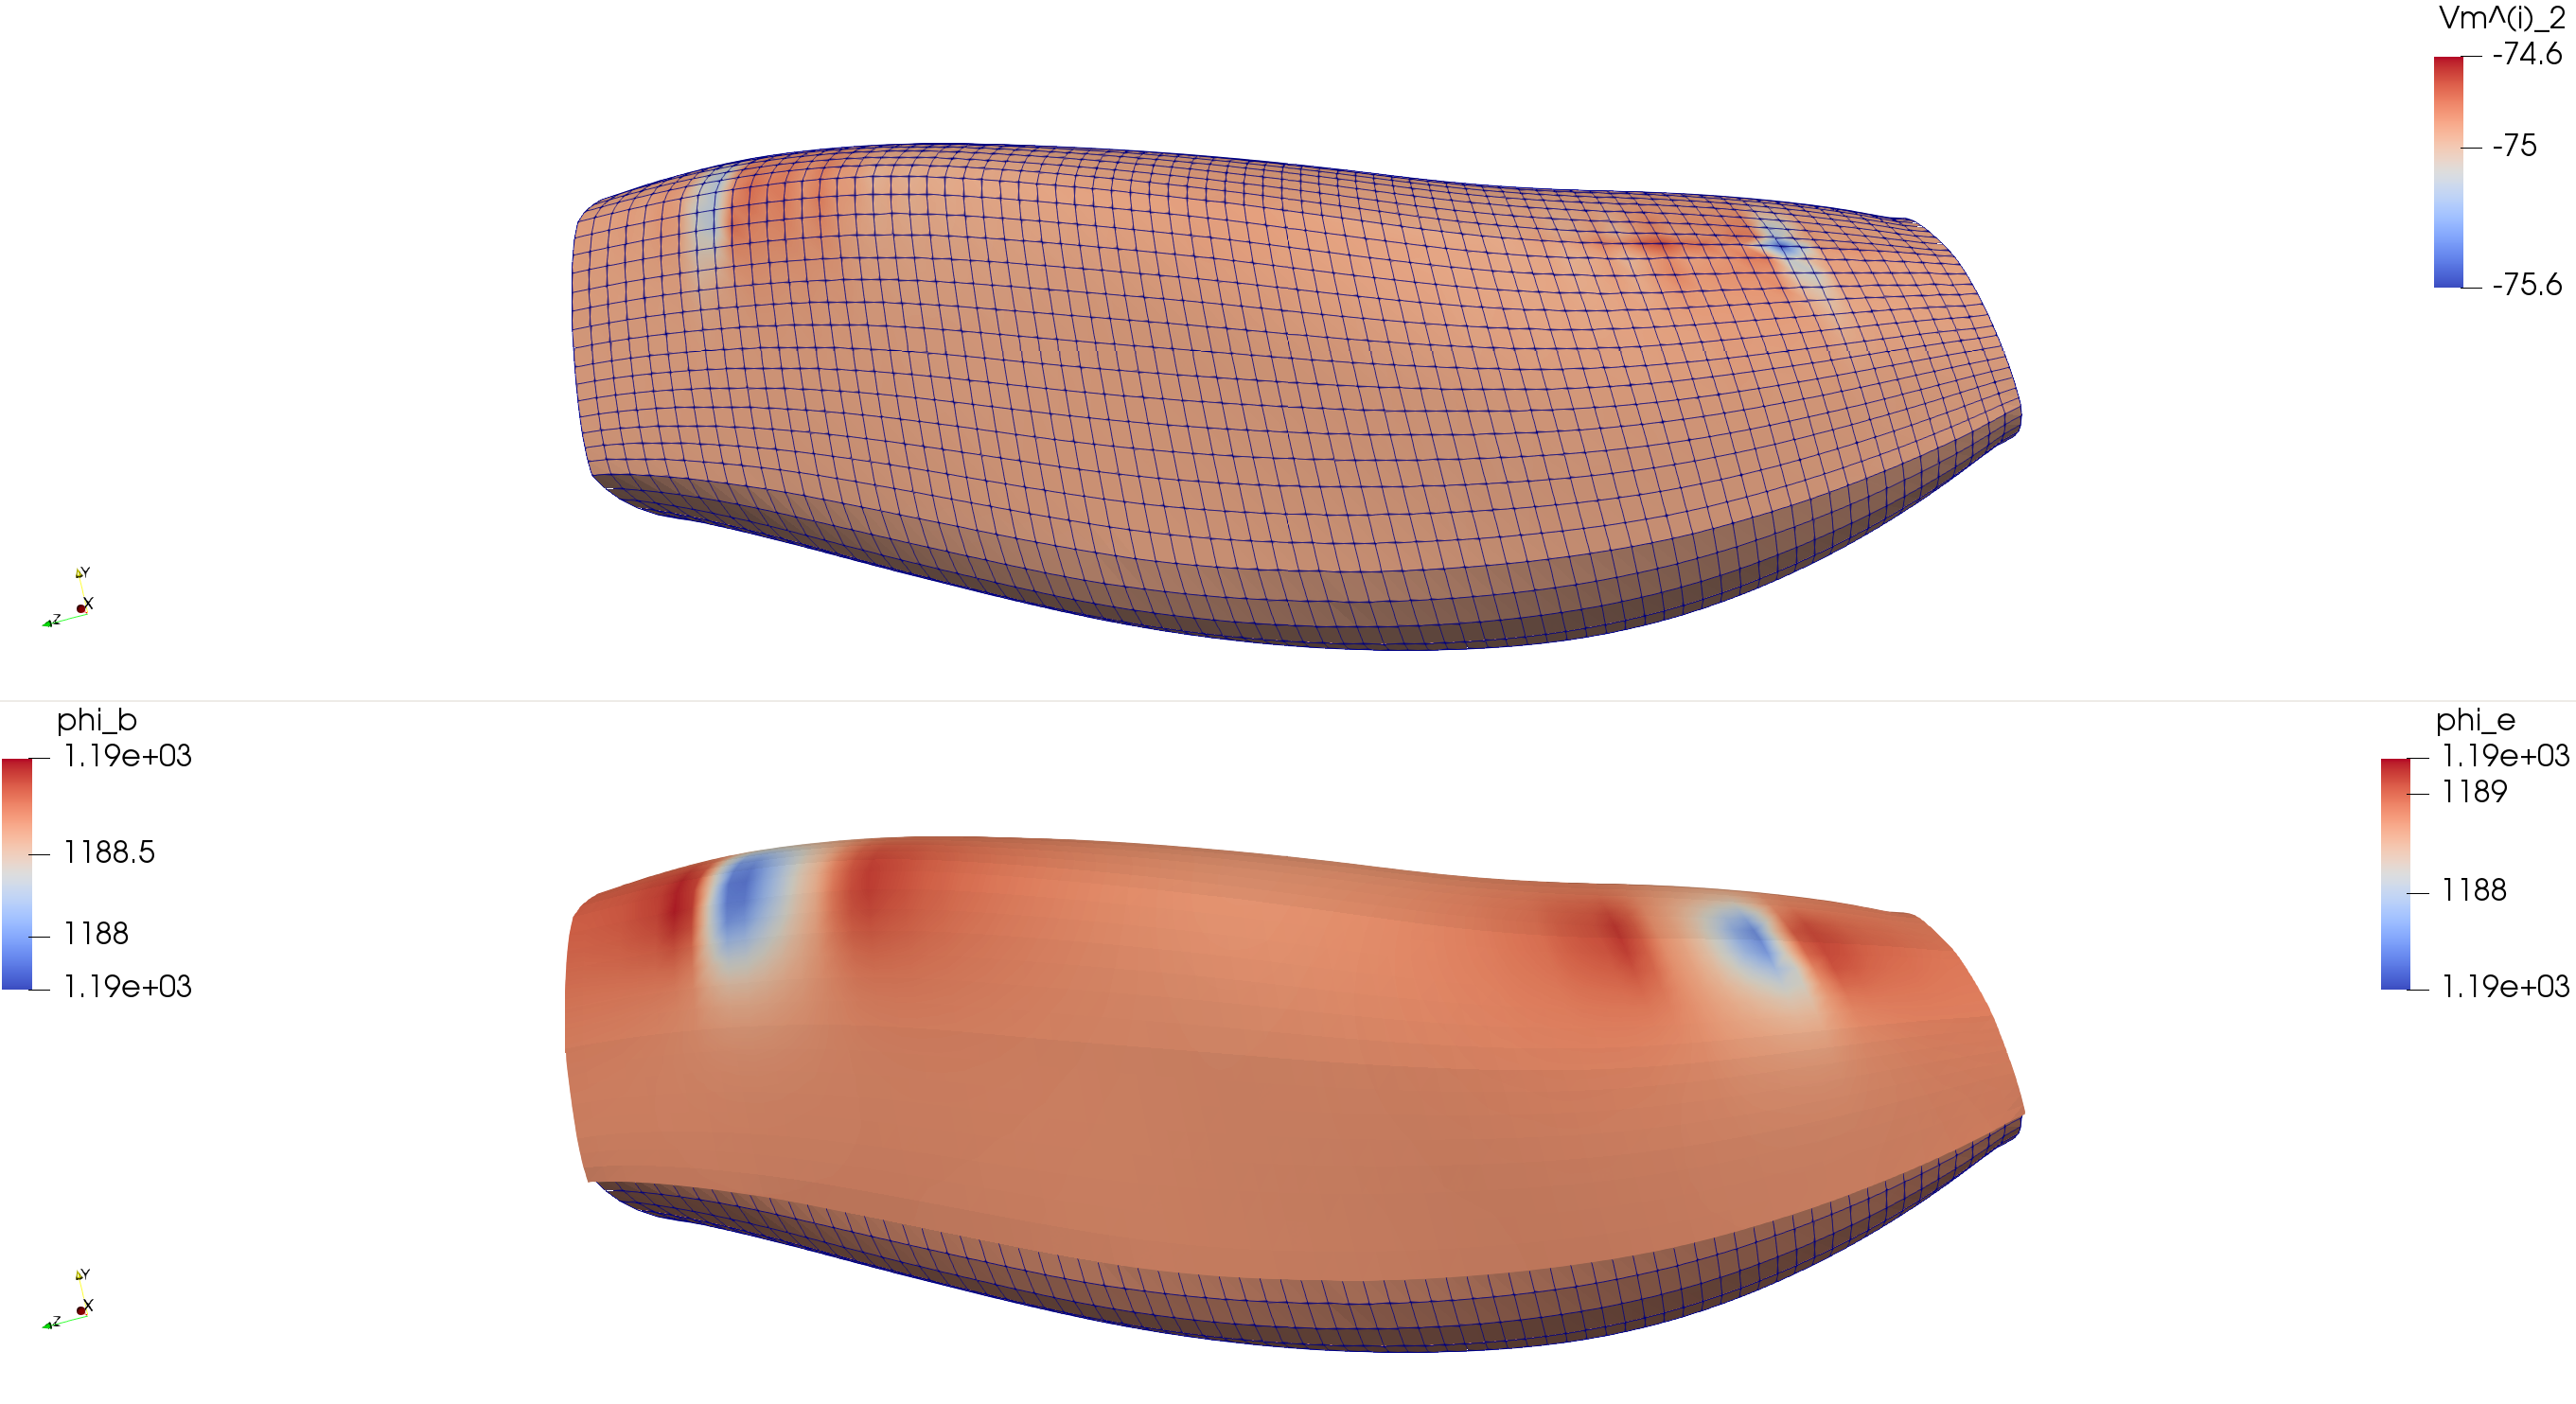
\includegraphics[width=\textwidth]{images/results/application/multidomain_Vm2_phi_b.png}%
    \caption{$V_m^2$ and $\phi_b$}%
    \label{fig:16_hodgkin_huxley_gpu}%
  \end{subfigure}   
  \caption{gpu.}%
  \label{fig:16_hodgkin_huxley_cpu_gpu}%
\end{figure}%

% fibers and multidomain
\begin{figure}[H]
  \centering%
  \begin{subfigure}[t]{0.48\textwidth}%
    \centering%
    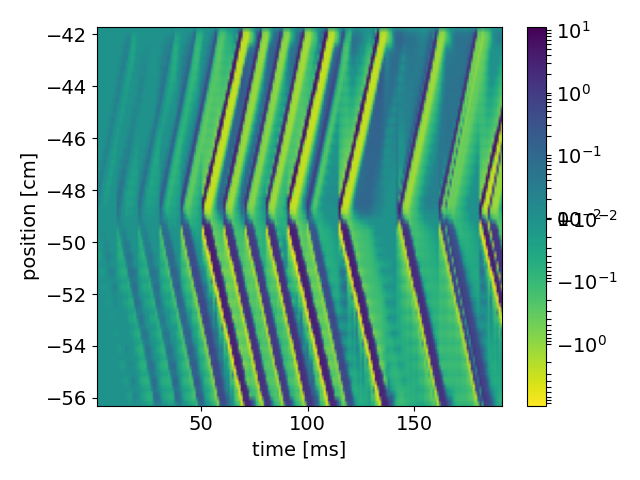
\includegraphics[width=\textwidth]{images/results/application/2_multidomain.png}%
    \caption{Multidomain}%
    \label{fig:2_multidomain}%
  \end{subfigure}
  \quad
  \begin{subfigure}[t]{0.48\textwidth}%
    \centering%
    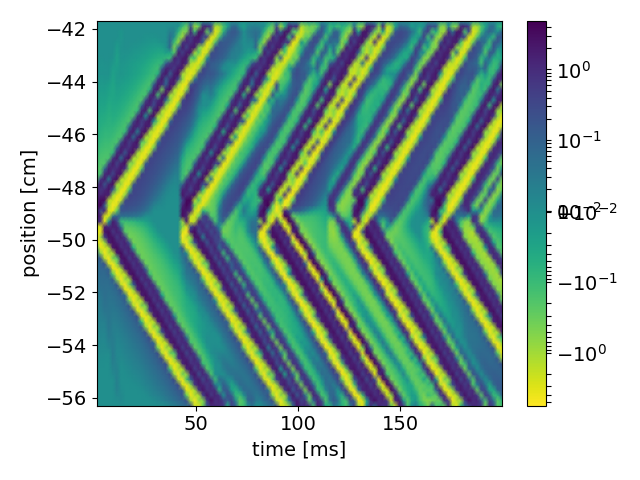
\includegraphics[width=\textwidth]{images/results/application/2_fibers.png}%
    \caption{Fibers}%
    \label{fig:2_fibers}%
  \end{subfigure}   
  \caption{Fibers and Multidomain}%
  \label{fig:multidomain_fibers}%
\end{figure}%


%-----
\section{Application: Linear mechanics with artifical electrophysiology}
%-----
\section{Application: Fibers and Muscle contraction, no-precice}
%-----

% prestretch
\begin{figure}[H]
  \centering%
  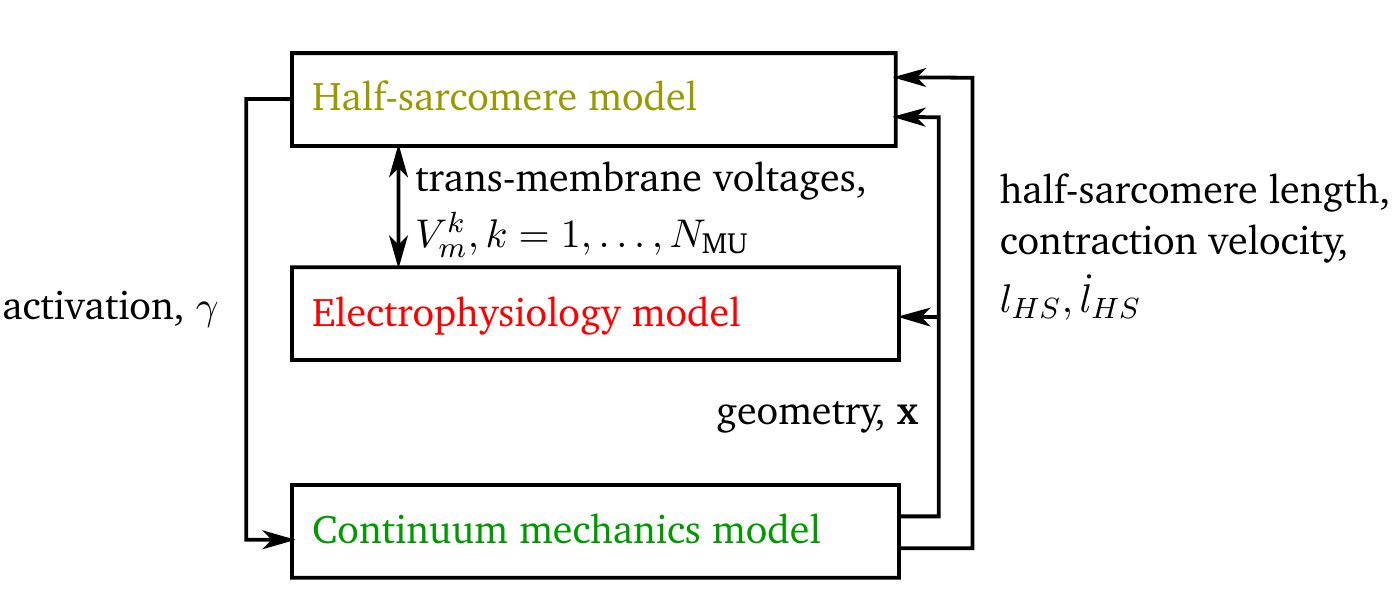
\includegraphics[width=0.5\textwidth]{images/results/application/fibers_muscle_contraction_quantities.png}%
  \caption{prestretch}%
  \label{fig:prestrech1b}%
\end{figure}%
\section{Application: Fibers and Muscle contraction, with tendons precice}

% muscle contraction
\begin{figure}
  \centering%
  \includegraphics[width=0.5\textwidth]{images/results/application/neuromuscular_muscle_contraction_traction.png}%
  \caption{solver structure}%
  \label{fig:neuromuscular_muscle_contraction_traction}%
\end{figure}%

%-----
\section{Application: Neuromuscular system with Spindles and Prestretch}

% prestretch
\begin{figure}[H]
  \centering%
  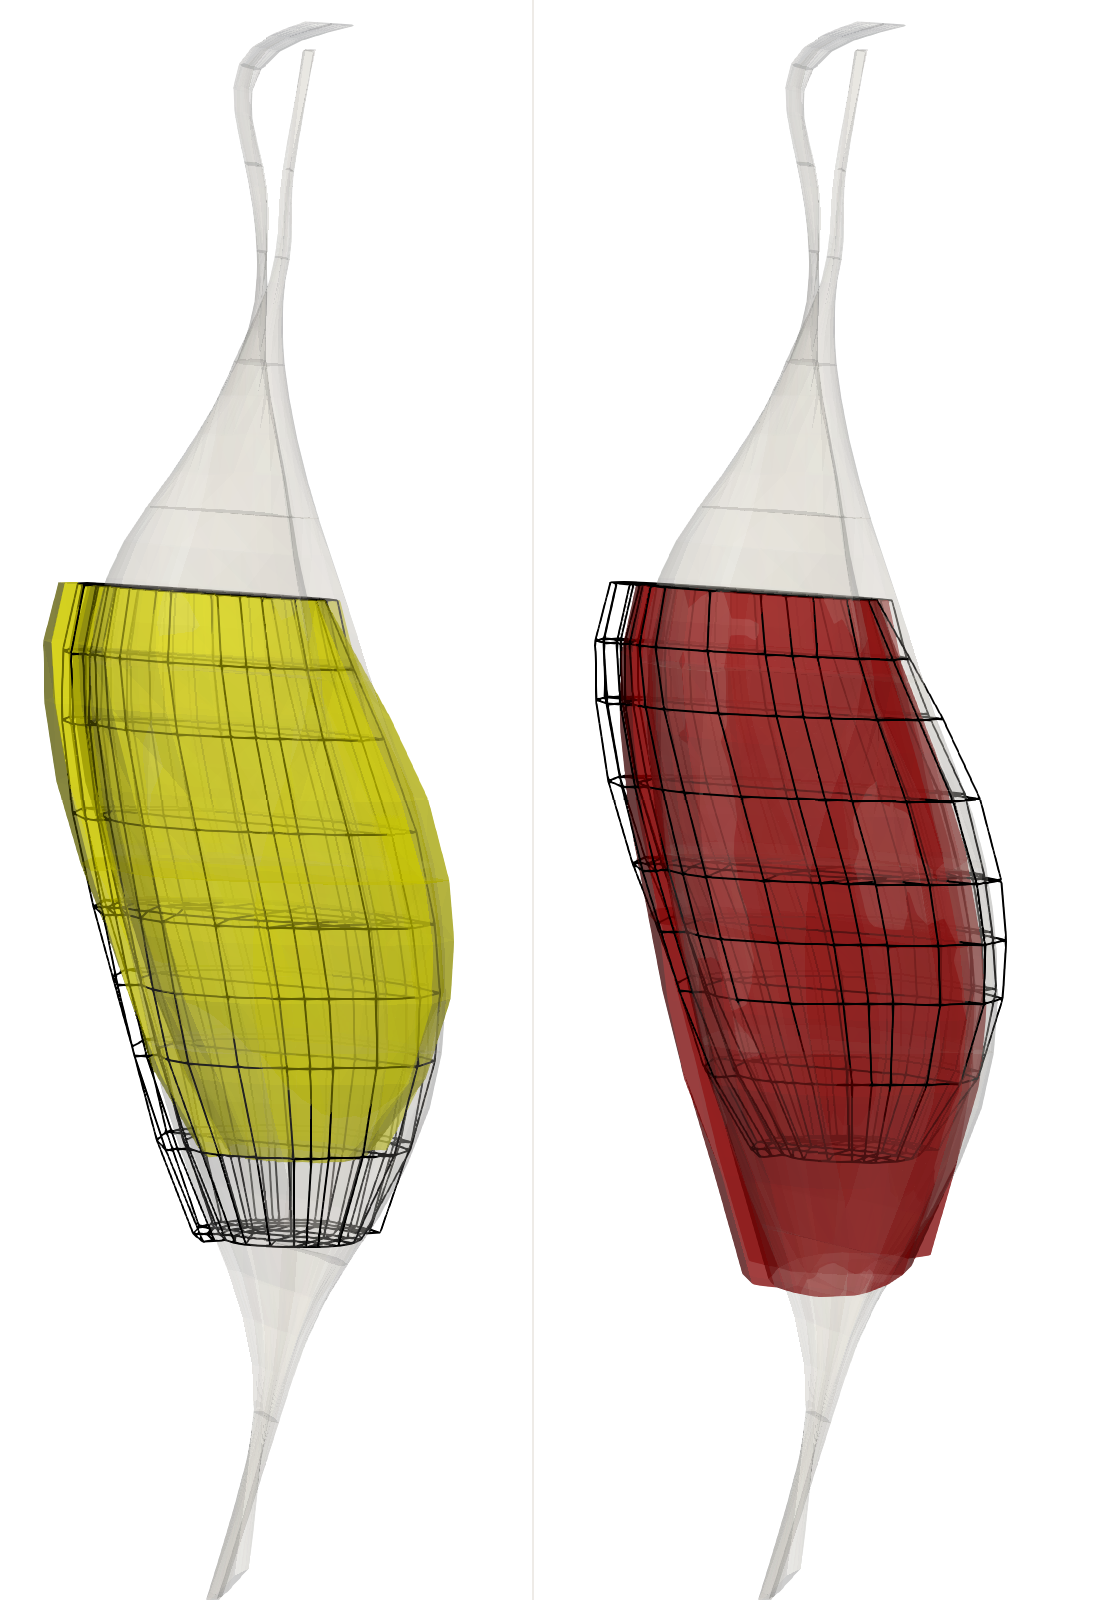
\includegraphics[width=0.5\textwidth]{images/results/application/neuromuscular_prestretch2c.png}%
  \caption{prestretch}%
  \label{fig:neuromuscular_prestretch2c}%
\end{figure}%

% image of contracting muscle
\begin{figure}[H]
  \centering%
  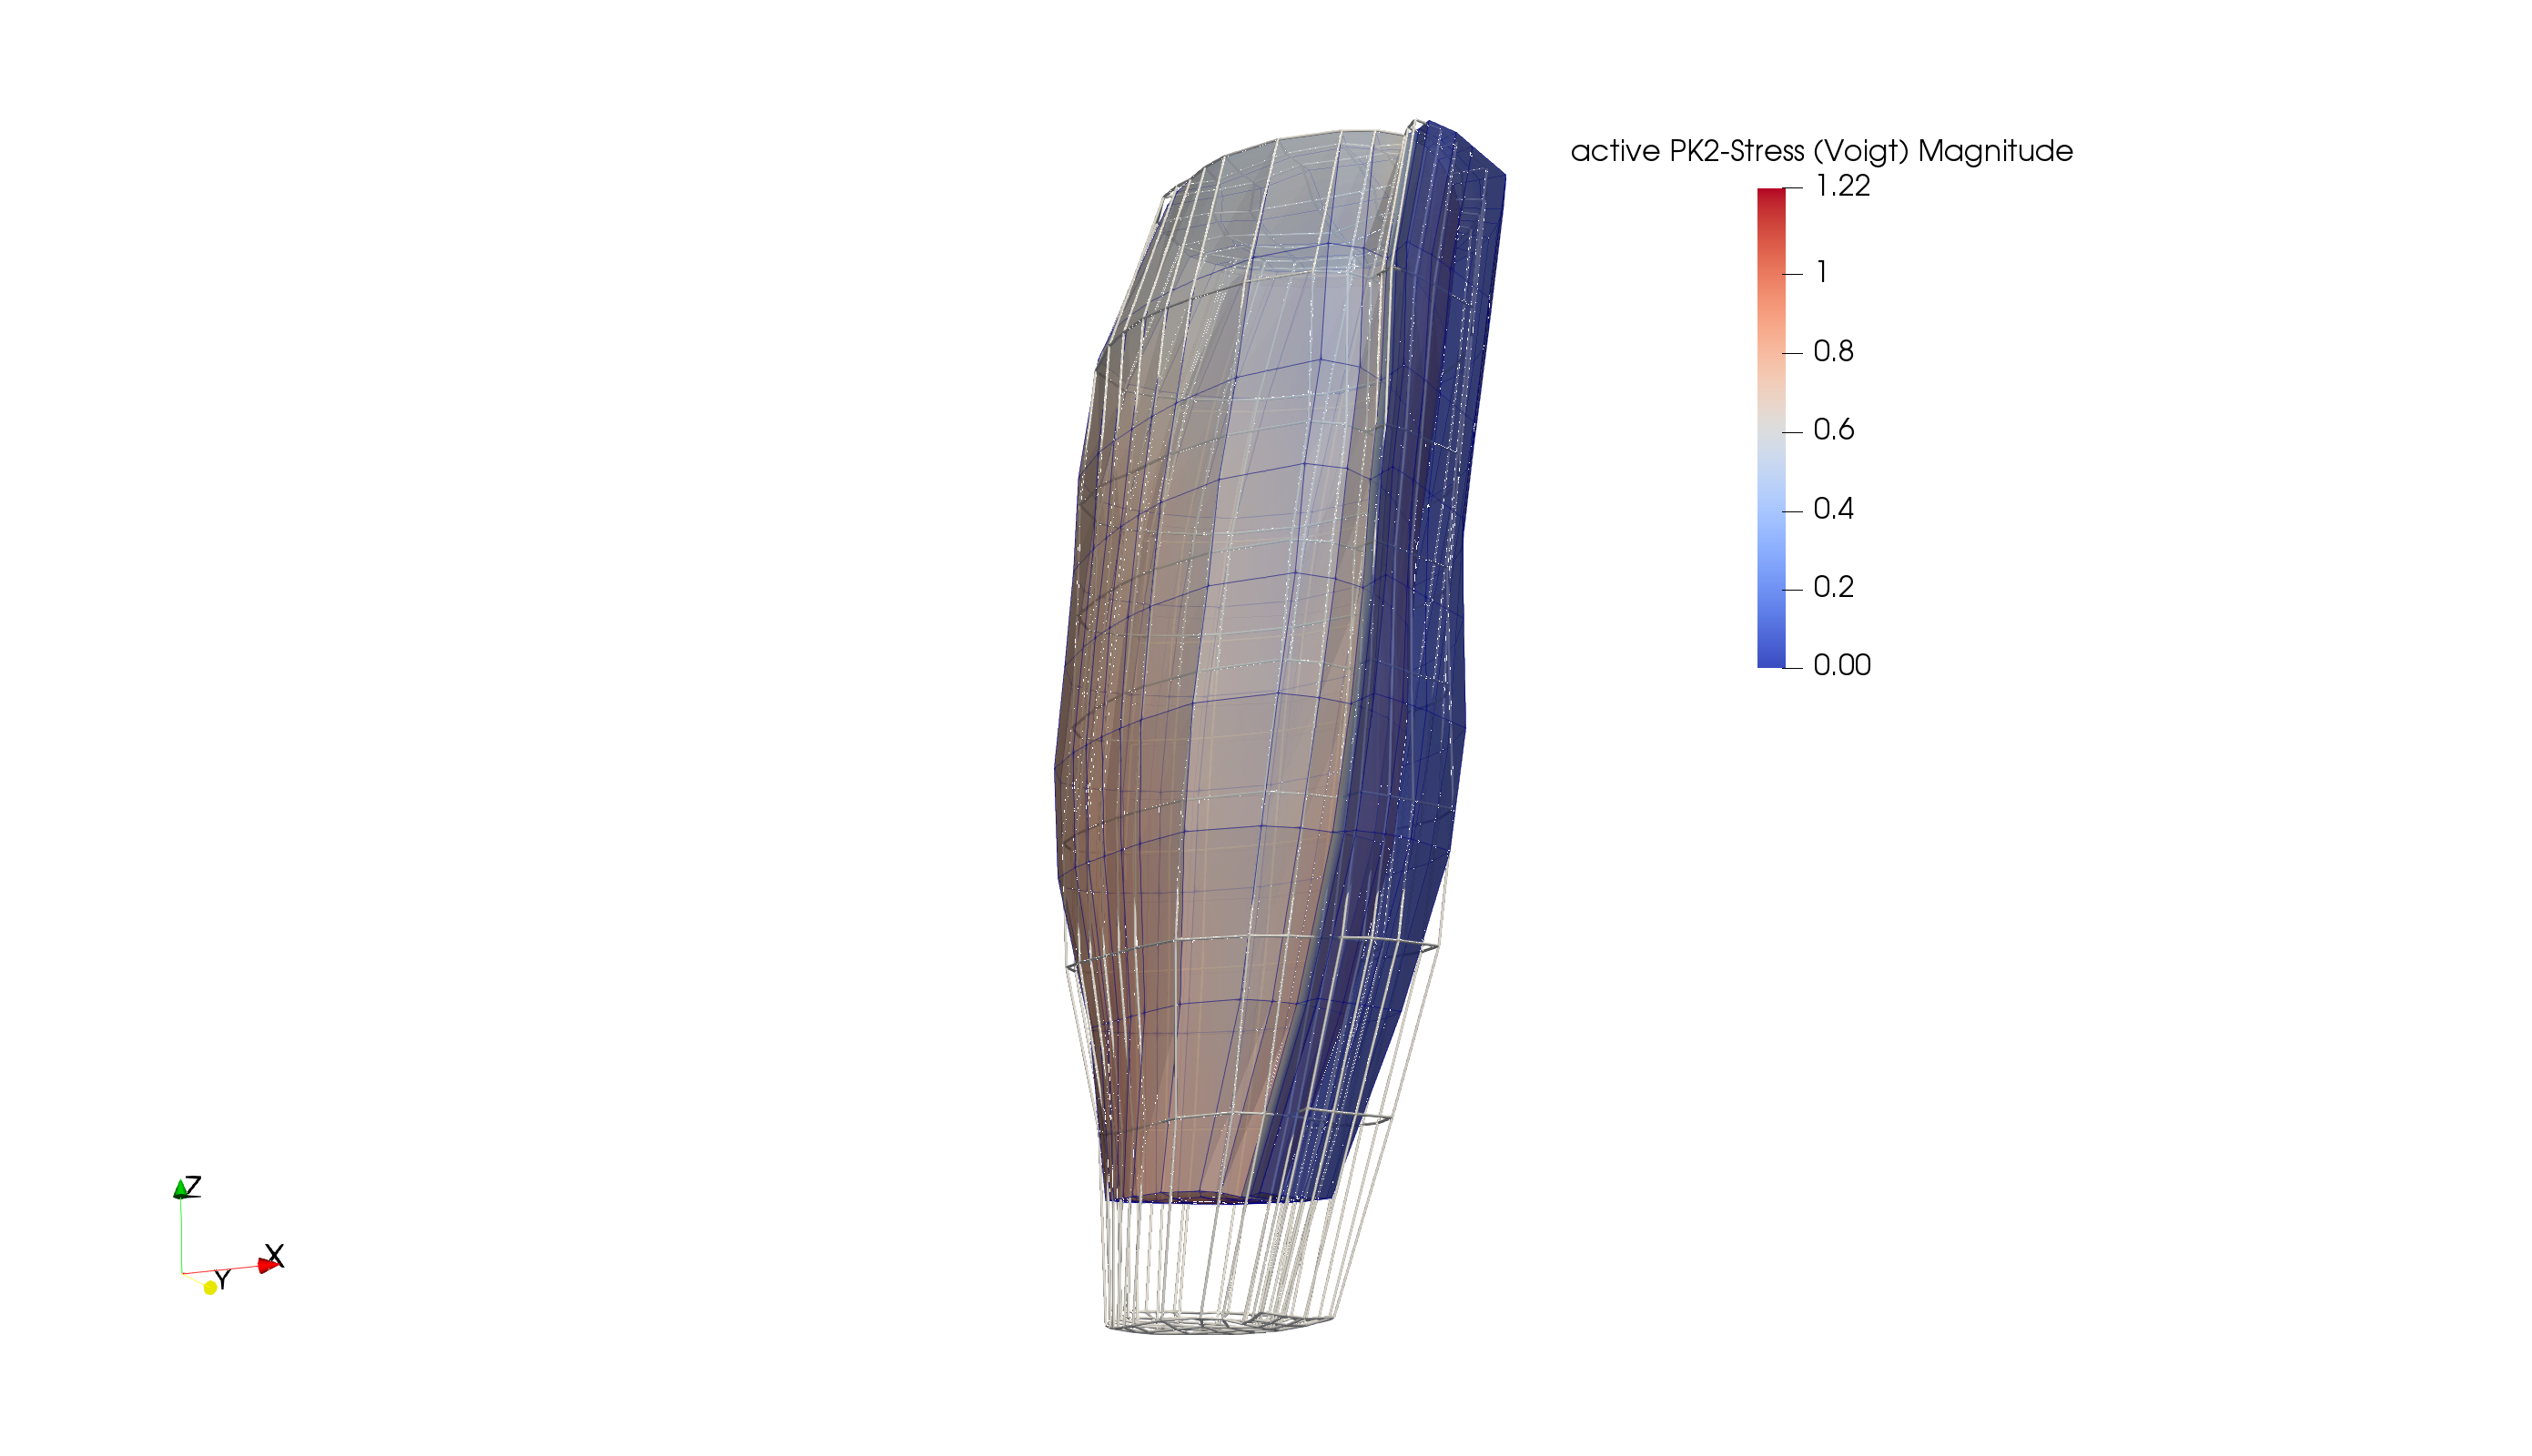
\includegraphics[width=\textwidth]{images/results/application/neuromuscular_contraction0.png}%
  \caption{Reference and current configuration.}%
  \label{fig:neuromuscular_contraction0}%
\end{figure}


% data flow of spindles
\begin{figure}[H]
  \centering%
  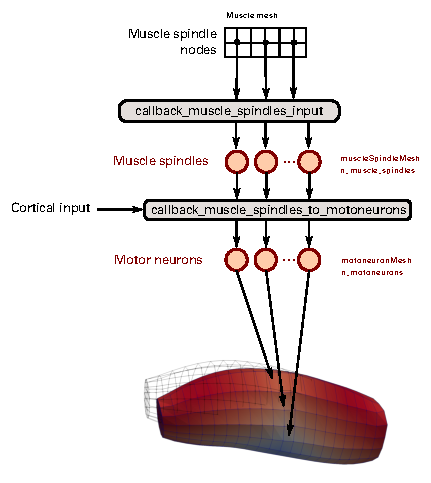
\includegraphics[width=\textwidth]{images/results/application/schematic_spindles.pdf}%
  \caption{Data flow of simulation with spindles and motor neurons}%
  \label{fig:neuromuscular_schematic}%
\end{figure}

% results
\begin{figure}[H]
  \centering%
  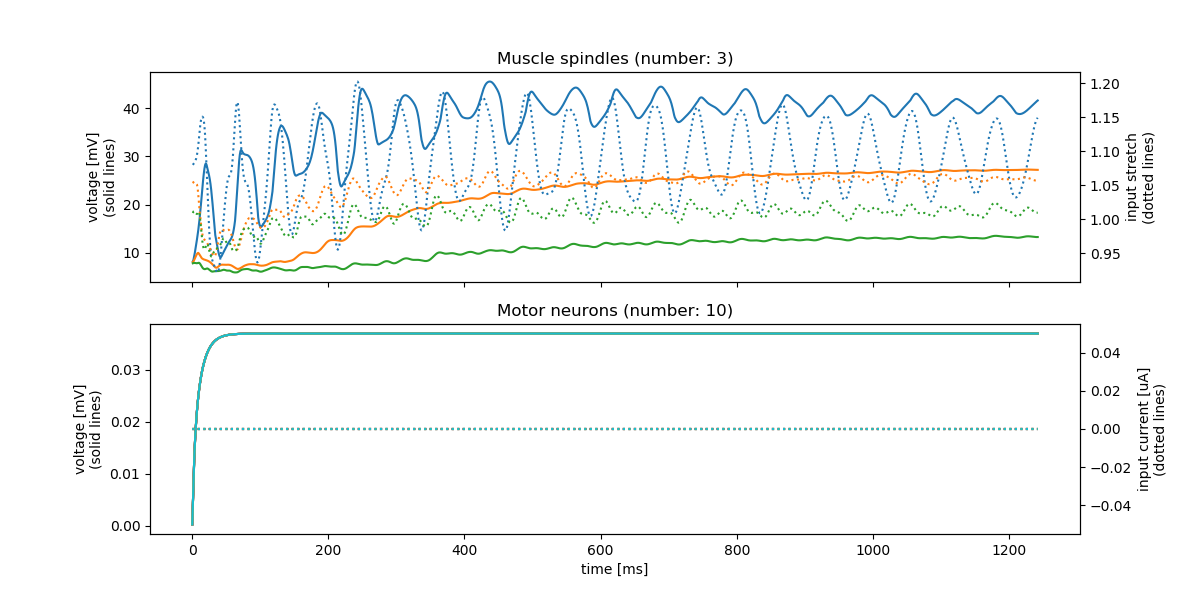
\includegraphics[width=\textwidth]{images/results/application/neuromuscular_spindle_out.png}%
  \caption{Activation data of sensors and neurons}%
  \label{fig:neuromuscular_schematic}%
\end{figure}

%-----
\section{Application: Neuromuscular system with More Sensor Organs}\label{sec:application_neuromuscular_system_more}

% data flow Golgi tendon organs
\begin{figure}[H]
  \centering%
  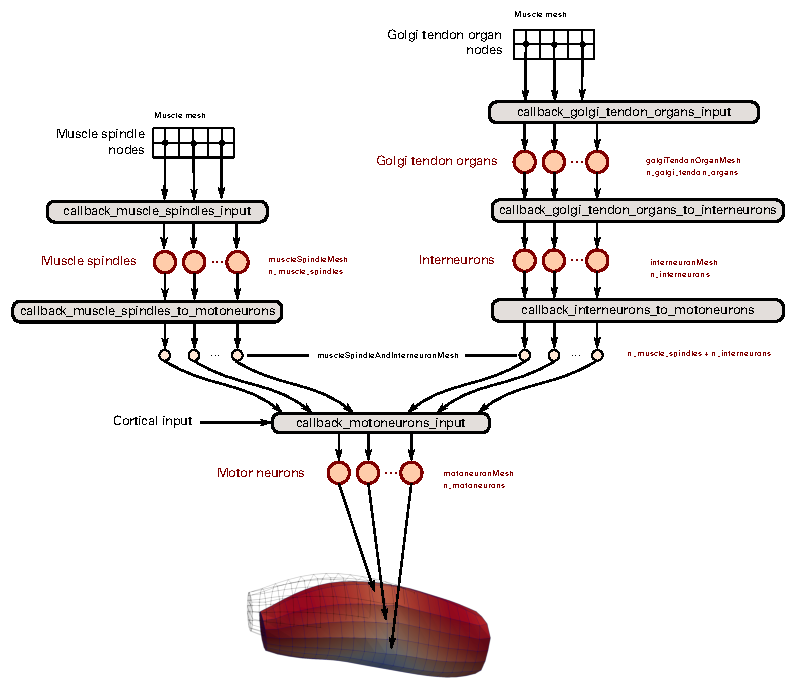
\includegraphics[width=\textwidth]{images/results/application/neuromuscular_schematic.pdf}%
  \caption{Data flow of simulation with spindles, Golgi tendon organs and motor neurons}%
  \label{fig:neuromuscular_schematic}%
\end{figure}

% results
\begin{figure}[H]
  \centering%
  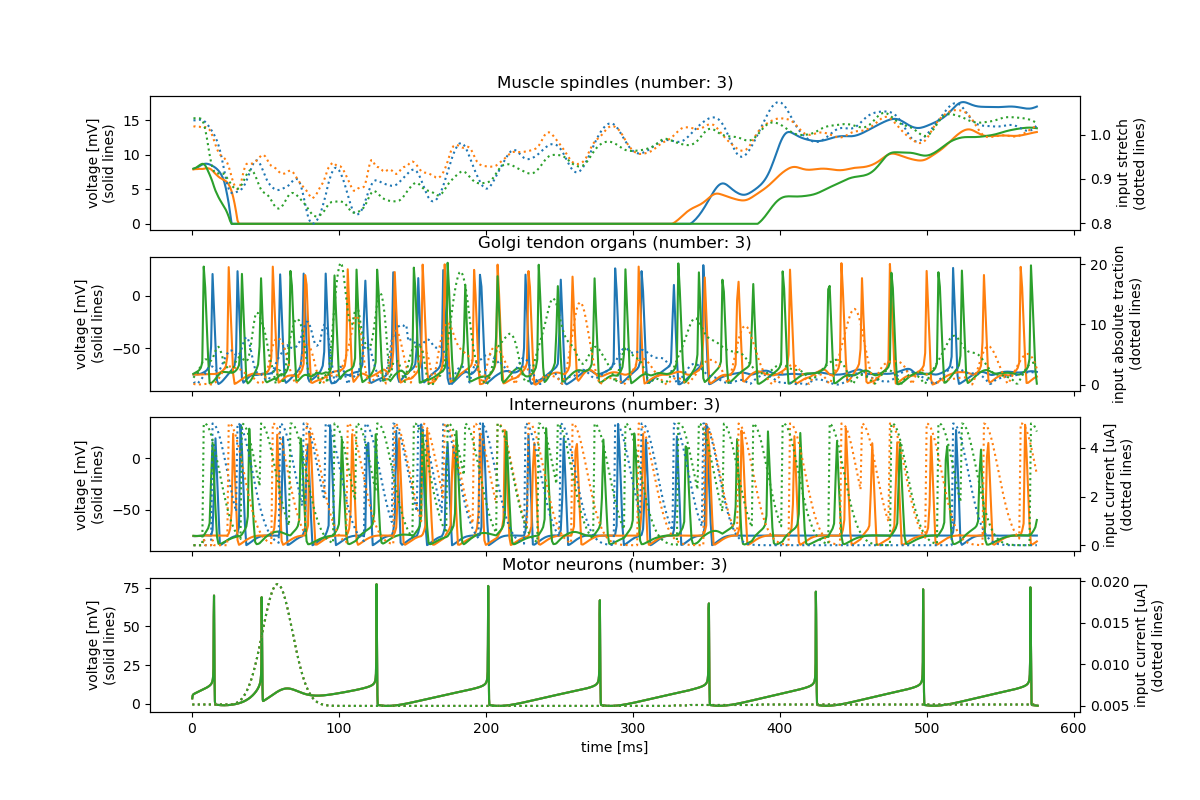
\includegraphics[width=\textwidth]{images/results/application/neuromuscular_mileusnic_out0.png}\\
  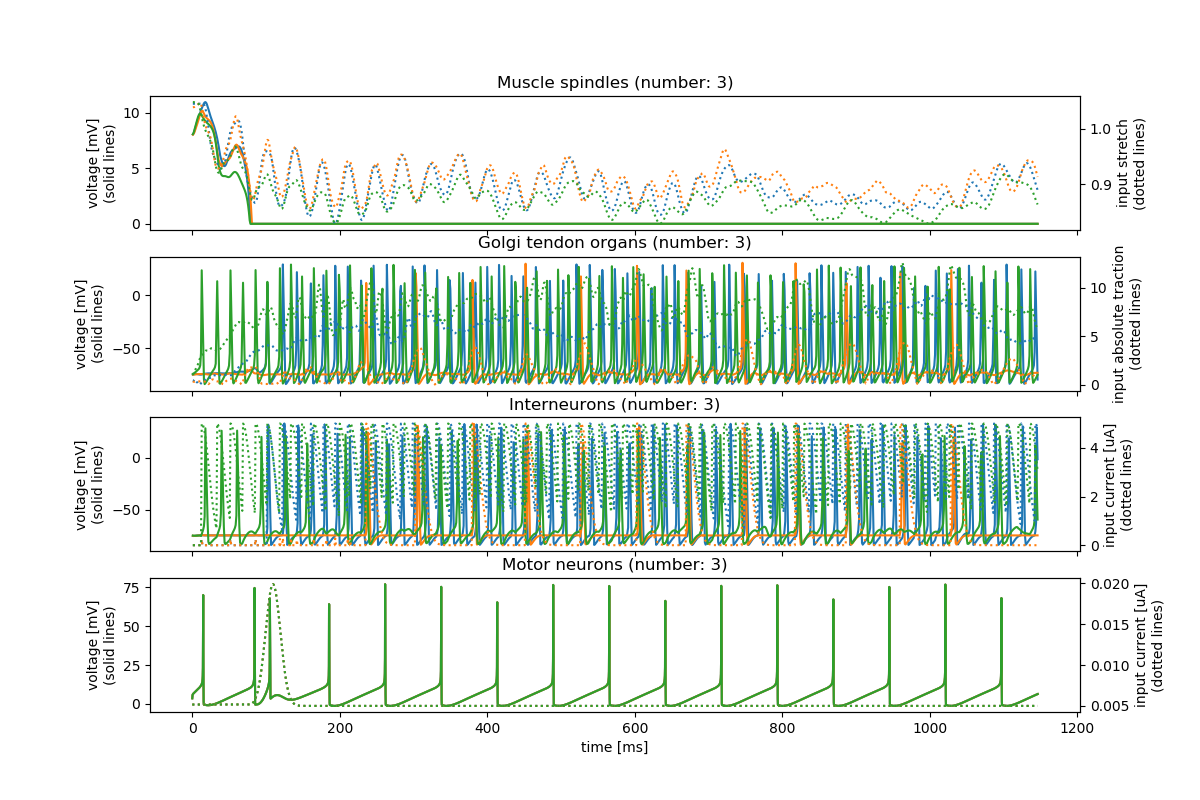
\includegraphics[width=\textwidth]{images/results/application/neuromuscular_mileusnic_out1.png}\\
  \caption{Activation data of sensors and neurons}%
  \label{fig:neuromuscular_schematic}%
\end{figure}

% --------------------------------
% studies
%-----
\section{Strang Splitting}
%-----
\section{Performance of OpenCMISS}

%-----
\section{Node level performance, roofline}

% weak scaling runtime
\begin{figure}[H]
  \centering%
  \begin{subfigure}[t]{0.48\textwidth}%
    \centering%
    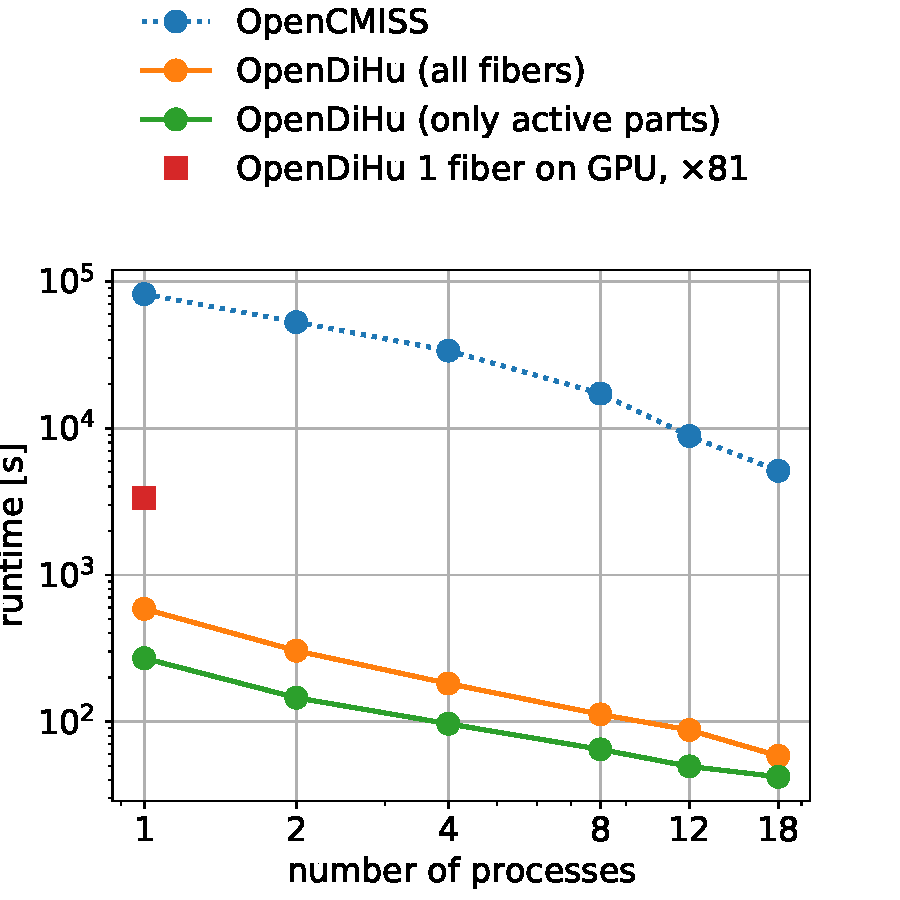
\includegraphics[width=\textwidth]{images/results/studies/0_weak_scaling_runtime.pdf}%
    \caption{a.}%
    \label{fig:16_hodgkin_huxley_cpu}%
  \end{subfigure}
  \quad
  \begin{subfigure}[t]{0.48\textwidth}%
    \centering%
    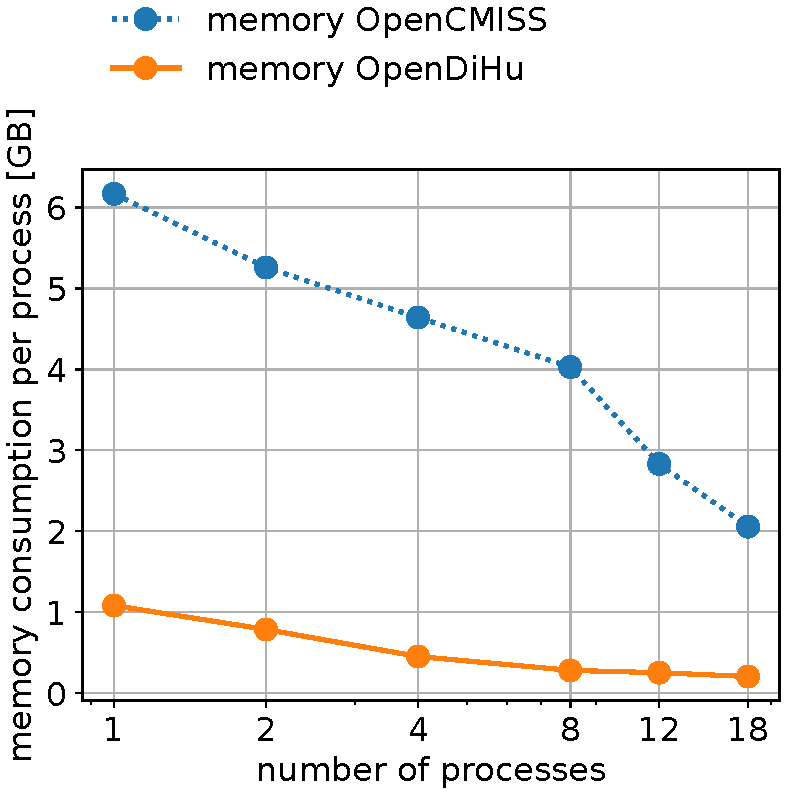
\includegraphics[width=\textwidth]{images/results/studies/0_weak_scaling_memory.pdf}%
    \caption{a.}%
    \label{fig:16_hodgkin_huxley_gpu}%
  \end{subfigure}   
  \caption{gpu.}%
  \label{fig:16_hodgkin_huxley_cpu_gpu}%
\end{figure}%

% weak scaling efficency
\begin{figure}[H]
  \centering%
  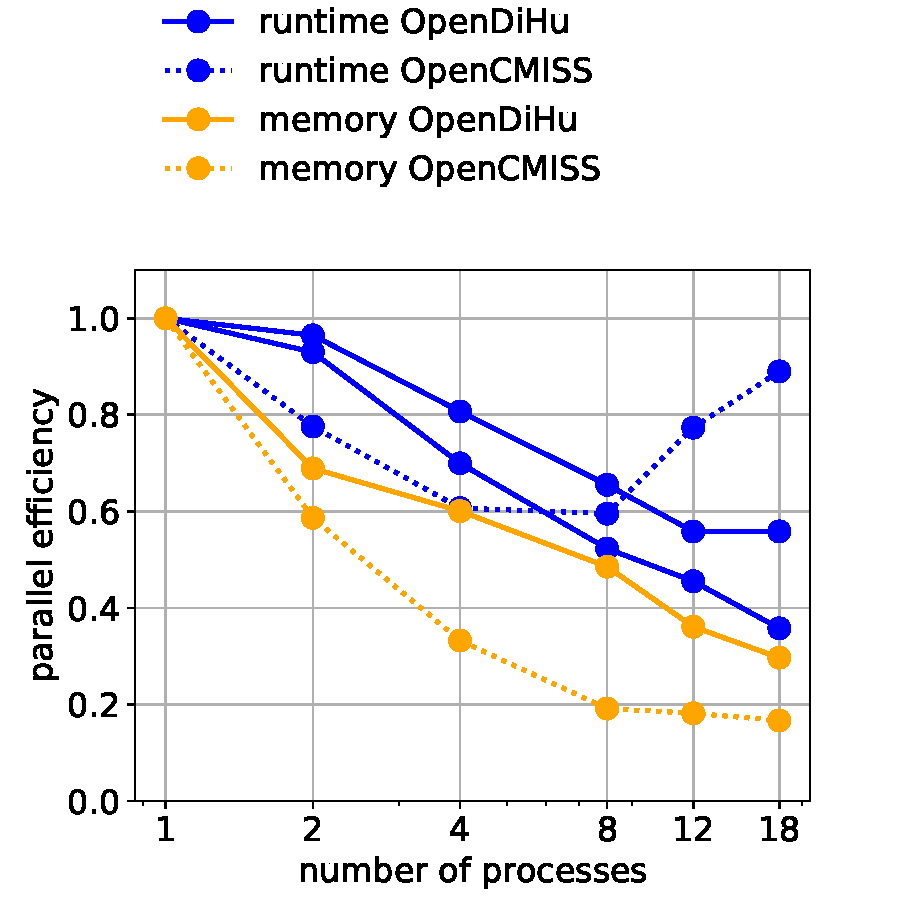
\includegraphics[width=\textwidth]{images/results/studies/0_weak_scaling_efficiency.pdf}%
  \caption{Efficiency model}%
  \label{fig:roofline}%
\end{figure}%

% roofline model
\begin{figure}[H]
  \centering%
  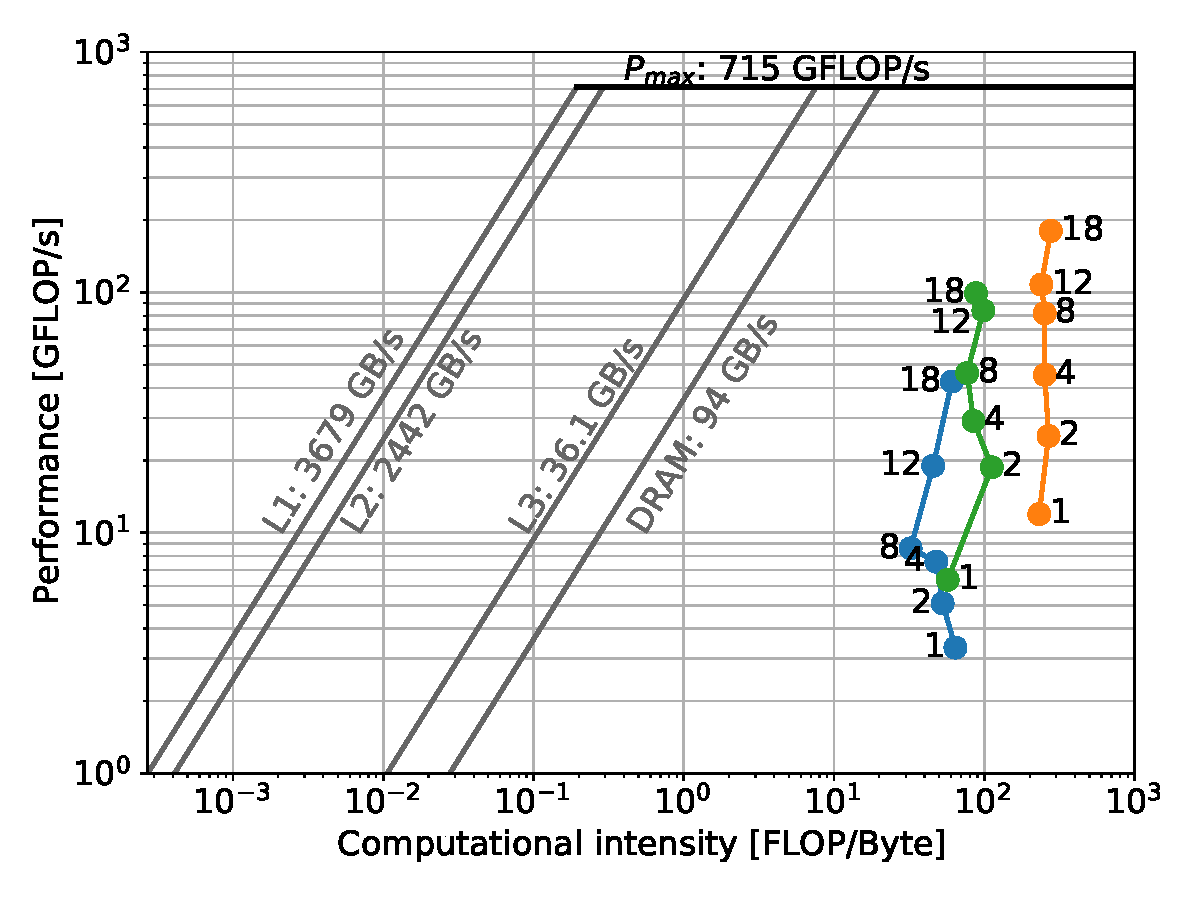
\includegraphics[width=\textwidth]{images/results/studies/0_roofline.pdf}%
  \caption{Roofline model}%
  \label{fig:roofline}%
\end{figure}%

%-----
\section{GPU}
\begin{figure}%
  \centering%
  \begin{subfigure}[t]{0.48\textwidth}%
    \centering%
    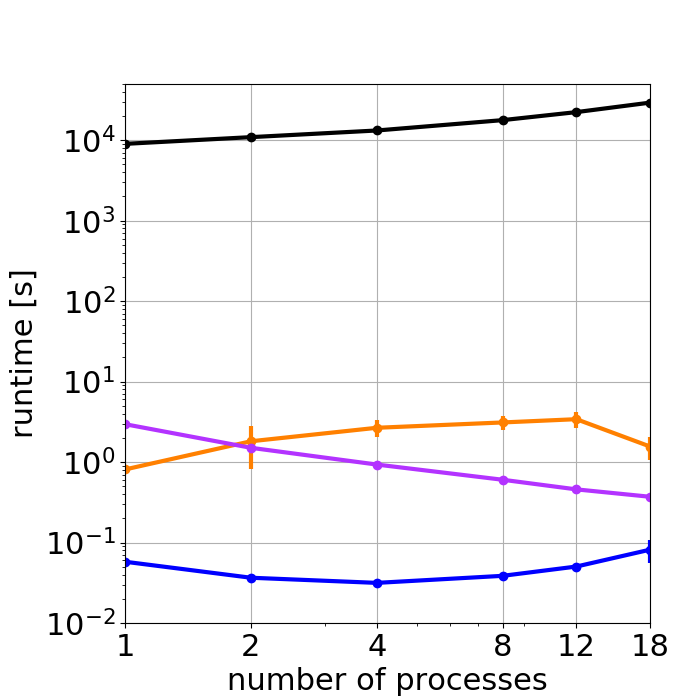
\includegraphics[height=6.5cm]{images/results/studies/16_hodgkin_huxley_gpu.png}%
    \caption{a.}%
    \label{fig:16_hodgkin_huxley_gpu}%
  \end{subfigure}
  \,
  \begin{subfigure}[t]{0.48\textwidth}%
    \centering%
    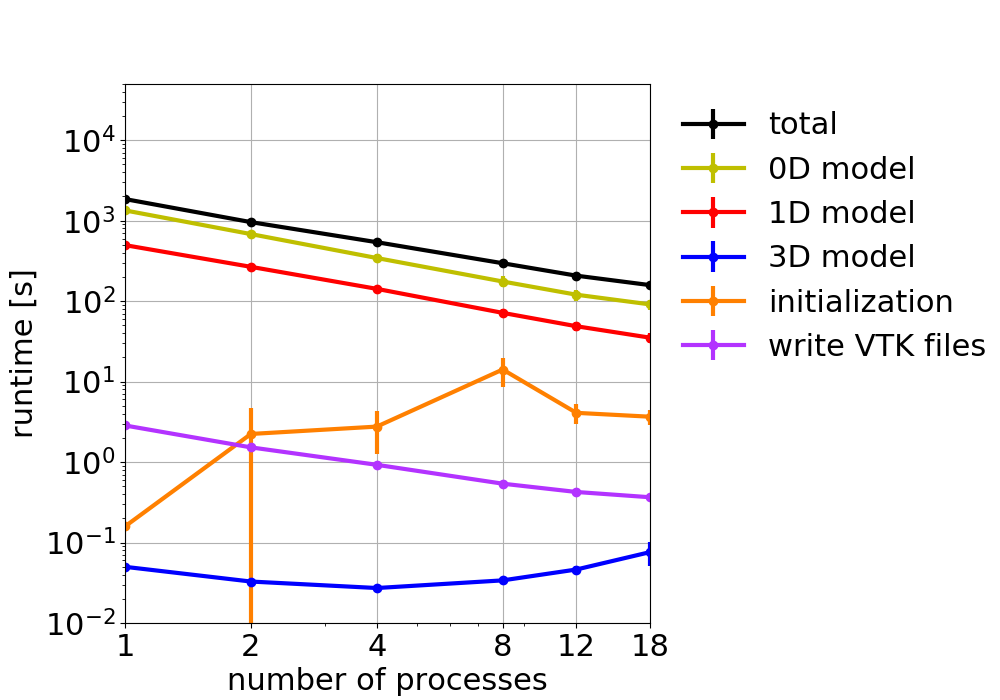
\includegraphics[height=6.5cm]{images/results/studies/16_hodgkin_huxley_cpu.png}%
    \caption{a.}%
    \label{fig:16_hodgkin_huxley_cpu}%
  \end{subfigure}   
  \caption{gpu.}%
  \label{fig:16_hodgkin_huxley_cpu_gpu}%
\end{figure}%



%-----
\section{OpenCMISS Godunov -> Strang}
%-----
\section{OpenCMISS linear solvers}
%-----
\section{OpenCIMSS total numer of elements per fiber}
%-----
\section{OpenCMISS strong scaling, weak scaling}
%-----
\section{OpenCMISS Domain decomposition shapes}
%-----
\section{Opendihu different compilers}
hlrs report, runtime of 0D 1D
%-----
\section{FastMonodomainSolver}
hlrs report
%-----
\section{Opendihu Weak scaling}
Hazel hen plot of coupled paper, new plots on hawk
% performance/opendihu/08_0D1D_better_implementation
%-----
\section{Opendihu rank placement strategies}

%-----
\section{Multidomain Solvers}

% linear solvers for multidomain
\begin{figure}[H]%
  \centering%
  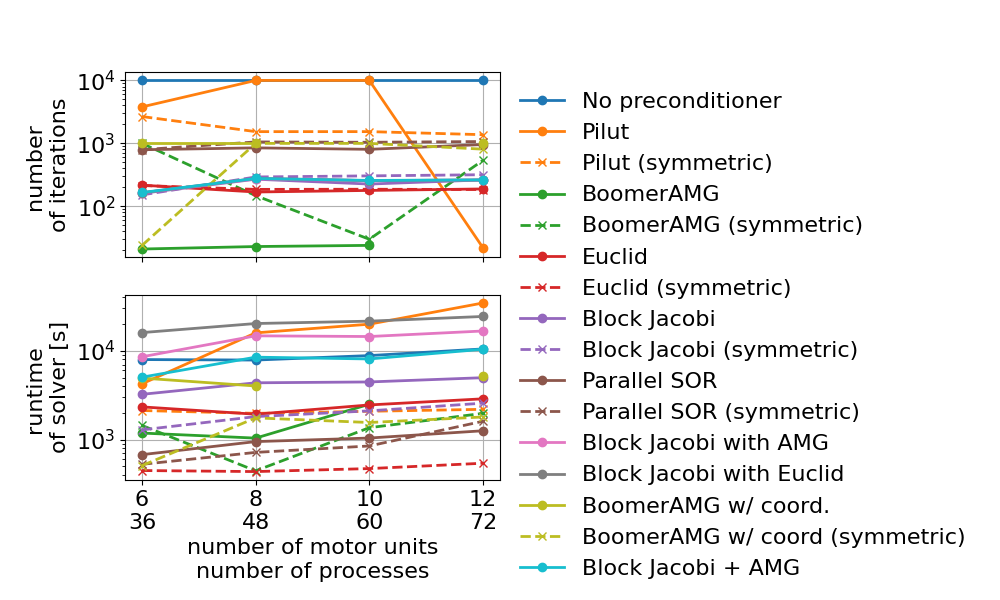
\includegraphics[width=\textwidth]{images/results/studies/multidomain_solvers_all.png}%
  \caption{Caption}%
  \label{fig:fig1}%
\end{figure}
%-----
\section{Output file sizes}
%-----
\section{Mesh convergence, stochastic with different MU assignments}
%-----
\section{dx-dt dependencies}
%performance/opendihu/03_dx_dt_dependence
%performance/opendihu/09_monodomain_dt0D_dt1D
%-----
\section{PinT}
%-----
\section{Load balancing}
%-----
\section{Application of opendihu within the field of robotics}

\chapter{Conclusion and Future Work}\label{sec:conclusion_and_future_work}

\section{Future Work}\label{sec:future_work}
 
% more timestepping methods: CVODE (https://computing.llnl.gov/projects/sundials/cvode), imex
% different parallelisation where not all ranks have to be involved (for multidomain) -> this feature already exists for the fibers with multipleInstances


%- end 




